\documentclass[12pt,twoside,final]{article}
\usepackage{comment}
\usepackage{adjustbox}
\usepackage[center]{caption}
\usepackage[portuguese,brazil]{babel}
\usepackage[utf8]{inputenc}
\usepackage{indentfirst}
\RequirePackage{etex}
\usepackage{hyperref,ae}
\usepackage{pslatex}
\usepackage{amssymb,fancyhdr,fancybox,epsfig,psfrag,amsmath,tabularx}
\usepackage[paperwidth=8.5in,paperheight=11in,hmargin={25mm,20mm},vmargin={20mm,20mm}]{geometry}
\usepackage{graphicx, url}
\usepackage{subfigure,tocloft}
\usepackage{changepage}
%\usepackage{subcaption}
\usepackage{float}
\usepackage[utf8]{inputenc}
\usepackage{mathtools} 
\usepackage{siunitx}
\usepackage{pgfplots}
\usepackage{etoolbox}
\usepgfplotslibrary{dateplot}
\pgfplotsset{compat=1.14}
%\usepackage{filecontents}
\usepackage{pgfplotstable}
\pgfplotsset{table/search path={csv}}
\usepackage{multirow}
\usepackage[lined,ruled,vlined,linesnumbered,portuguese]{algorithm2e}
\usepackage{ulem,soul}
\usepackage[section]{placeins}
\usepackage[dvips]{lscape} %rotacionar
\usepackage{setspace}

\usepackage{listings}
\usepackage{needspace}

\lstset{
    basicstyle=\ttfamily\small,
    columns=fullflexible,
    keepspaces=true,
    breaklines=true,
    breakatwhitespace=true,
    showstringspaces=false,
    aboveskip=10pt,
    belowskip=10pt
}
\renewcommand{\lstlistingname}{Código}
\renewcommand{\lstlistlistingname}{Lista de Códigos}
\usepackage{wrapfig, graphics,multirow}
\usepackage{array}
\usepackage{pdfpages}
\usepackage{pdflscape}
\usetikzlibrary{matrix}
\usepackage{enumitem,comment}  
\usepackage[titletoc,title]{appendix}
\renewcommand{\cfttoctitlefont}{\hspace*{\fill}\large\bfseries\MakeUppercase}
\renewcommand{\cftaftertoctitle}{\hspace*{\fill}}
\renewcommand{\cftlottitlefont}{\hspace*{\fill}\large  \bfseries}
\renewcommand{\cftafterlottitle}{\hspace*{\fill}}
\renewcommand{\cftloftitlefont}{\hspace*{\fill}\large \bfseries}
\renewcommand{\cftafterloftitle}{\hspace*{\fill}}
\usepackage[Lenny]{fncychap}
\setlength{\headheight}{15pt}
\setlength{\parindent}{1.2cm}

\usepackage{xcolor}
\definecolor{azure}{rgb}{0.0, 0.5, 1.0}
\newcommand{\blue}[1]{\textcolor{azure}{#1}}
\newcommand{\strikeRed}[1]{\textcolor{red}{\sout{#1}}}
\newcommand{\red}[1]{\textcolor{red}{#1}}
\newcommand{\green}[1]{\textcolor{green}{#1}}


\usepackage{longtable}
\usepackage{rotating}
%\usepackage[dvipsnames]{xcolor}
\usepackage{lscape}

%\usepackage[ngerman]{babel}
\usepackage[num,abnt-repeated-author-omit=yes,abnt-emphasize = bf]{abntex2cite}
\citebrackets[]
\renewcommand{\sectionmark}[1]{\markright{\thesection. \ #1}}
\fancyhead{}
\fancyfoot{}
\fancyhead[RE,RO]{\thepage}
\renewcommand{\headrulewidth}{0pt}
\hyphenation{pro-fis-si-o-nais}
%\hyphenation{ín-di-ce}


\newcolumntype{P}[1]{>{\centering\arraybackslash}P{#1}}


\renewcommand{\listtablename}{LISTA TABELAS} 
\renewcommand{\listfigurename}{LISTA  FIGURAS}

\newcolumntype{M}[1]{>{\centering\arraybackslash}m{#1}}


\usepackage{color, colortbl}
\newcommand{\dbh}[1]{\textcolor{blue}{#1}}
\newcommand{\bac}[1]{\textcolor{red}{#1}}

\newenvironment{widerequation}{%
    \begin{adjustwidth}{-3cm}{-1.5cm}\begin{equation}}
    {\end{equation}\end{adjustwidth}}


\begin{document}


\thispagestyle{empty}

%PPC em português
%================================================================================================
%================================= PRIMEIRA FOLHA INTERNA  ======================================
%================================================================================================
\begin{figure}
\center

\includegraphics[height=0.15\textwidth]{Figs/logoCefetCampusPetropolis.jpg} 
\end{figure}


\vspace*{0.8cm}

\begin{center}
{\large \bf CENTRO FEDERAL DE EDUCAÇÃO TECNOLÓGICA} \vspace{1mm} \\
{\large \bf CELSO SUCKOW DA FONSECA - CEFET/RJ \textit{CAMPUS} PETRÓPOLIS} \vspace{1mm} \\
{\large \bf CURSO: BACHARELADO EM ENGENHARIA DE COMPUTAÇÃO}\\

\vspace*{5cm}
{\large \bf \blue{[ToDo:] Título do trabalho.}}\\
\end{center}
\vspace{4cm}
\hfill
%\begin{minipage}%{0.45\linewidth}
	\begin{flushright}
	{ Jonatas Halliday Sant Anna do Nascimento}
	\end{flushright}
%\end{minipage}


\vspace*{3.3cm}
\begin{center}
{\bf PETRÓPOLIS \\{ 2026}}\\
\end{center}

%--------------------------------------------------------------------------
%--------------------------------------------------------------------------
\newpage
\pagestyle{empty}

\begin{center}
{\large \bf CENTRO FEDERAL DE EDUCAÇÃO TECNOLÓGICA} \vspace{1mm} \\
{\large \bf CELSO SUCKOW DA FONSECA - CEFET/RJ \textit{CAMPUS} PETRÓPOLIS} \vspace{1mm} \\
{\large \bf CURSO: BACHARELADO EM ENGENHARIA DE COMPUTAÇÃO}

\vspace*{3cm}
\normalsize{\large \bf \blue{[ToDo:] Título do trabalho.}}\\
\end{center}
\vspace{1.5cm}
\hfill
%\begin{minipage}%{0.45\linewidth}
	\begin{flushright}
	\blue{Jonatas Halliday Sant Anna do Nascimento}
	\end{flushright}
%\end{minipage}
\vspace*{1.5cm}
\begin{flushright}
	\begin{minipage}{0.5\textwidth}
		{\normalsize
		Trabalho de Conclusão de Curso apresentado ao  
	 CEFET/RJ - {\it campus} Petrópolis, como parte dos requisitos para obtenção do título de Bacharel em Engenharia de Computação.}
	\end{minipage}\\[1.5cm]
\end{flushright}
\vspace{1.5cm}
\hfill
%\begin{minipage}%{0.45\linewidth}
\begin{flushright}
\blue{[ToDo:] Orientadora: Professor(a) Nome do Professor(a)}\\
\blue{[ToDo:] Coorientador: Professor(a) Nome do Professor(a)}
\end{flushright}




\vspace*{3.3cm}
\begin{center}
{\bf PETRÓPOLIS \\ \blue{[ToDo:] Ano}}\\
\end{center}



%--------------------------------------------------------------------------
%--------------------------------------------------------------------------
\newpage
\begin{minipage}{0.9\textwidth}

{\normalsize 
\begin{center}
Autorizo a reprodução e divulgação total ou parcial deste trabalho, por qualquer meio eletrônico ou convencional, para fins de estudo e pesquisa, desde que citada a fonte.
\end{center}
\vspace*{0.5cm}
}
\end{minipage}
\vspace*{5cm}
\begin{center}
\blue{[ToDo:] Acrescentar ficha catalográfica (providenciada pela biblioteca) após a defesa do TCC.}
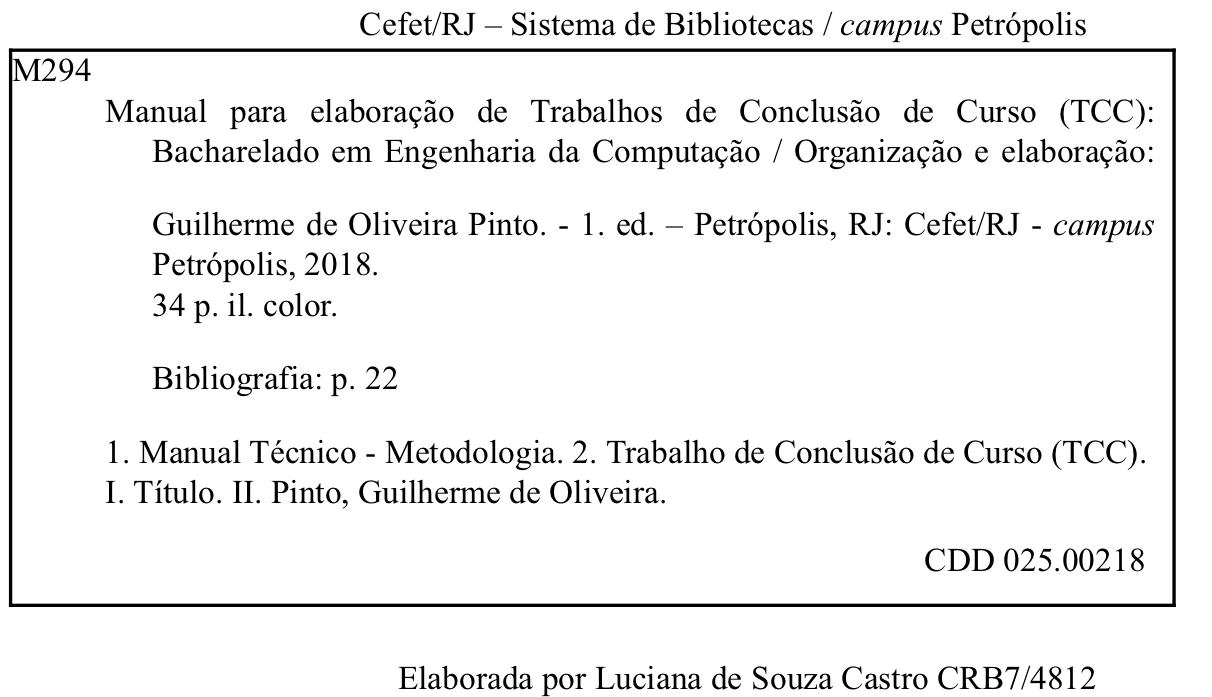
\includegraphics[height=0.5\textwidth]{Figs/biblioteca_engcomp.jpeg}
\end{center}


%--------------------------------------------------------------------------
%--------------------------------------------------------------------------

\newpage
\newcommand{\HRule}{\rule{0.6\linewidth}{0.5mm}}
\pagestyle{empty}

{\center % Center everything on the page


\begin{figure}
\center

\includegraphics[height=0.13\textwidth]{Figs/logoCefetCampusPetropolis.jpg} 
\end{figure}

\begin{center}
{\large \bf CENTRO FEDERAL DE EDUCAÇÃO TECNOLÓGICA} \vspace{1mm} \\
{\large \bf CELSO SUCKOW DA FONSECA - CEFET/RJ \textit{CAMPUS} PETRÓPOLIS} \vspace{1mm} \\
{\large \bf CURSO: BACHARELADO EM ENGENHARIA DE COMPUTAÇÃO}\\
\vspace*{1.2cm}
{\large  FOLHA DE APROVAÇÃO}

\vspace*{1.3cm}
{\large \bf \blue{[ToDo:] Título do trabalho.}}\\
\end{center}
\vspace{0.5cm}
\hfill
%\begin{minipage}%{0.45\linewidth}
\begin{flushright}
    \blue{Jonatas Halliday Sant Anna do Nascimento}
	\end{flushright}
%\end{minipage}
\vspace*{0.5cm}
\begin{flushright}
	\begin{minipage}{0.5\textwidth}
		{\normalsize
		Trabalho de Conclusão de Curso apresentado ao  
	 CEFET/RJ -{ {\it campus} Petrópolis}, como parte dos requisitos para obtenção do título de Bacharel em Engenharia de Computação.}
	\end{minipage}\\[0.5cm]
\end{flushright}
\vspace{0.5cm}
\hfill
%\begin{minipage}%{0.45\linewidth}
\begin{flushright}
\blue{[ToDo:] Orientador(a): Nome do Professor(a)} \\
\blue{[ToDo:] Corientador(a): Nome do Professor(a)} \\
\end{flushright}

\begin{minipage}{0.9\textwidth}
	\begin{flushleft}
	Aprovado por:
	\end{flushleft}
\end{minipage}\\[1cm]

\center
\HRule \\
\blue{[ToDo:] Nome do Professor(a)} \\[0.4cm]
\HRule \\
\blue{[ToDo:] Nome do Professor(a)} \\[0.4cm]
\HRule \\
\blue{[ToDo:] Nome do Professor(a)} \\[0.4cm]
\HRule \\
\blue{[ToDo:] Nome do Professor(a)} \\[1.2cm]


\begin{center}
\blue{[ToDo:] Mês de Ano}
\end{center}


}



\newpage


\begin{center}
\textbf{\large DEDICATÓRIA}
\end{center}
      \vspace{0.5cm}

\blue{[ToDo: ] Escrever dedicatória.}

\newpage



% Agradecimento
\begin{center}
\textbf{\large  AGRADECIMENTO}
\end{center}
      \vspace{0.5cm}
      
\blue{[ToDo: ] Escrever agradecimento.}


\newpage


% Resumo
\begin{center}
\textbf{\large RESUMO}
\end{center}
      \vspace{0.5cm}
      
      
   \blue{[ToDo: ] Escrever resumo em português}\\
    
    
      
      
      
\begin{flushleft}
\textbf{Palavras-Chave: \blue{[ToDo: ] Escrever palavras-chave em português.}}
\end{flushleft}

\newpage

\begin{center}
\textbf{\large ABSTRACT}
\end{center}
\vspace{0.5cm}

 \blue{[ToDo: ] Escrever resumo em inglês}\\

\begin{flushleft}
\textbf{Palavras-Chave: \blue{[ToDo: ] Escrever palavras-chave em inglês.}}
\end{flushleft}









\newpage

%=============================== lista de tabelas e figuras ==========================
{\thispagestyle{empty}
\renewcommand{\listfigurename}{LISTA DE FIGURAS}

\listoffigures}
\newpage

{\thispagestyle{empty}
\renewcommand{\listtablename}{LISTA DE TABELAS}
\listoftables}
\newpage

\section*{Lista de Siglas}

\singlespacing

\blue{[ToDo: ] Escrever lista de siglas / acrónimos.}\\

\noindent
\begin{tabular}{l c p{.85\linewidth}}

TCC & - & Trabalho de Conclusão de Curso \\
CEFET & - & Centro Federal de Educação Tecnológica \\
RNA & - & Rede Neural Artificial \\
LSTM & - & \textit{Long Short-Term Memory} \\
VADER & - & \textit{Valence Aware Dictionary and sEntiment Reasoner} \\
NLP & - & \textit{Natural Language Processing} \\
ReLU & - & \textit{Rectified Linear Units} \\
MSE & - & \textit{Mean Squared Error} \\
MAE & - & \textit{Mean Absolute Error} \\
RMSE & - & \textit{Root Mean Squared Error} \\
RNN & - & \textit{Recurrent Neural Network} \\
MLP & - & \textit{Multi Layer Perceptron} \\
SVM & - & \textit{Support Vector Machine} \\
NB & - & \textit{Naive Bayes} \\
SRM & - & \textit{Structural Risk Minimization} \\
TF-IDF & - & \textit{Term Frequency-Inverse Document Frequency} \\
AMV & - & \textit{Amazon Mechanical Turk} \\
%% talvez tirar estas abaixo
LIWC & - & \textit{Linguistic Inquiry Word Count} \\
GI & - & \textit{General Inquirer} \\
ANEW & - & \textit{Affective Norms for English Words} \\
SWN & - & \textit{SentiWordNet} \\
SCN & - & \textit{SentiCNet} \\
WSD & - & \textit{Word-Sense Disambiguation} \\
%% talvez tirar estas acima
CNN & - & \textit{Convolutional Neural Network} \\
GSE & - & \textit{Ghana Stock Exchange} \\

\end{tabular}

\onehalfspacing
\clearpage

\section*{Lista de Símbolos}

\singlespacing

\noindent
\begin{tabular}{l c p{.85\linewidth}}

$\Omega$ & - & Espaço amostral \\

$\mathcal{F}$ & - & $\sigma$-álgebra \\

$\mathcal{F}_t$ & - & Informação disponível até o instante $t$ \\

$\mathbb{P}$ & - & Medida de probabilidade \\

$S_t$ & - & Preço do ativo subjacente no instante $t$ \\

$S_0$ & - & Preço inicial do ativo subjacente \\

$K$ & - & Preço de exercício (\textit{strike price}) \\

$T$ & - & Tempo até o vencimento da opção \\

$r$ & - & Taxa de juros livre de risco \\

$\mu$ & - & Taxa média de crescimento (\textit{drift}) \\

$\sigma$ & - & Volatilidade do ativo subjacente \\

$W_t$ & - & Movimento browniano no instante $t$ \\

$dW_t$ & - & Incremento do movimento browniano \\

$V(S,t)$ & - & Valor da opção em função do preço do ativo e do tempo \\

$C$ & - & Preço da opção de compra (\textit{call}) \\

$P$ & - & Preço da opção de venda (\textit{put}) \\

$d_1$ & - & Primeiro termo auxiliar da fórmula de Black--Scholes \\

$d_2$ & - & Segundo termo auxiliar da fórmula de Black--Scholes \\

$\Delta$ & - & Delta da opção \\

$\Gamma$ & - & Gamma da opção \\

$\Theta$ & - & Theta da opção \\

$\nu$ & - & Vega da opção \\

$\rho$ & - & Rho da opção \\

\end{tabular}

\clearpage

\newpage

%=============================== sumário =============================================

\tableofcontents

\newpage

\pagestyle{fancy}
\pagenumbering{arabic}
\onehalfspacing

\newpage
%=============================== capítulos ==========================================

\section{Introdução}
A modelagem matemática desempenha um papel fundamental nas finanças quantitativas ao fornecer ferramentas rigorosas, como a teoria da probabilidade e o cálculo estocástico, para representar a evolução temporal de variáveis sujeitas à incerteza de mercado. A importância dessa formalização torna-se ainda mais evidente na análise de  derivativos financeiros, cujos valores presentes são determinados por outros ativos financeiros, chamados de ativos subjacentes.
Entre os derivativos mais negociados globalmente, o mercado de opções ocupa uma posição de destaque \cite{fia2026options}. Por concederem ao seu detentor o direito, não a obrigação, de negociar um ativo a um preço fixado em uma data futura, as opções apresentam uma estrutura não linear de ganhos que as torna essenciais para a transferência e mitigação de riscos em carteiras de investimento. Segundo dados divulgados pela Futures Industry Association (FIA, 2026), aproximadamente 28,61 bilhões de contratos de opções foram negociados mundialmente no primeiro trimestre de 2026, em comparação com 9,74 bilhões de contratos futuros. Esses números evidenciam a relevância desse segmento no mercado internacional de derivativos negociados em bolsa. Essa flexibilidade contratual, associada à incerteza em relação a evolução futura dos preços dos ativos subjacentes, torna a precificação de opções um problema relevante para finanças quantitativas. Nesse quadro, o modelo desenvolvido por Black e Scholes \cite{blackscholes1973} estabeleceu uma fórmula fechada para determinar o preço teórico das opções de compra e venda europeias sob determinadas condições de mercado.

O modelo tem como base a representação do preço do ativo como um processo estocástico através do movimento browniano geométrico, assumindo parâmetros como volatilidade e taxa livre de juros constantes. Ao partir do objetivo da construção de uma carteira de proteção, ou também conhecido como carteira de \textit{Hedge}, continuamente ajustada e da ausência de arbitragem, obtém-se uma equação diferencial parcial em que a solução permite determinar o valor teórico do derivativo. Nesse cenário, a precificação passa a ser fundamentada em uma relação matemática entre as características do contrato, como o tempo até o seu fim, denominado de maturação, e toda a dinâmica envolvida na precificação desse ativo.

Para opções europeias de compra e venda, a formulação fornece expressões analíticas que relacionam o preço da opção ao valor corrente do ativo, ao preço de exercício, ao tempo restante até o vencimento, à taxa livre de risco e à volatilidade. Além de fornecer uma expressão para o preço teórico das opções, o modelo de Black-Scholes permite investigar a influência de seus parâmetros sobre o valor do derivativo, por meio das sensibilidades financeiras conhecidas como Gregas. A existência de uma formulação analítica possibilita, ainda, examinar as propriedades matemáticas da função de precificação, tornando o modelo uma referência para a avaliação de métodos computacionais de aproximação.

A existência dessa solução analítica permite utilizar o modelo como referência para a investigação de métodos computacionais capazes de aproximar relações matemáticas entre variáveis do problema. Nesse quadro, pode-se destacar a regressão simbólica como uma técnica avançada em aprendizado de máquina que utiliza programação genética e algoritmos evolutivos para identificar expressões matemáticas explícitas a partir dos dados, além de buscar aproximações numéricas que possibilitam investigar estruturas matemáticas e relações subjacentes aos dados. A regressão simbólica foi projetada para inferir expressões matemáticas interpretáveis orientada a dados, diferente de métodos cuja estrutura é previamente estabelecida. Entre as ferramentas disponíveis para essa finalidade, destaca-se o algoritmo PySR, que emprega técnicas da já mencionada busca evolutiva e aprendizado por árvores de decisão para identificar expressões simbólicas capazes de representar as relações presentes nos dados. Sua aplicação a uma função analítica conhecida, como a de Black-Scholes, permite investigar não apenas a capacidade de aproximação dos preços, mas também a correspondência entre as expressões identificadas e as propriedades matemáticas do modelo original.

\subsection{Tema}

\subsection{Justificativa}

\subsection{Delimitação}

\subsection{Objetivos}
Investigar a capacidade da regressão simbólica, por meio do algoritmo PySR, de aproximar a função de precificação de Black-Scholes, avaliando a precisão preditiva, a complexidade simbólica e a recuperação de propriedades matemáticas do modelo.

\subsection{Descrição resumida da metodologia}

\subsection{Descrição}
          % Introdução

\section{Fundamentos da precificação de opções}
\label{chapter:chapterName}

A dinâmica de preços do mercado financeiro é regida por diferentes e variados fatores. A modelagem do comportamento dos ativos financeiros busca representar a evolução de grandezas cujo comportamento futuro está sujeito à incerteza, como preços de ações, taxas de juros e volatilidade. No mercado de derivativos, essa característica assume particular importância, uma vez que o valor desses instrumentos depende da dinâmica de outro ativo, chamado de ativo subjacente.

A avaliação desses contratos depende, portanto, do comportamento do preço do ativo subjacente ao longo do tempo. Como sua evolução futura é de uma dinâmica estocástica uma carteira de \textit{hedge} visa mitigar os efeitos dessas oscilações ajustando dinâmicamente a proporção de opções presentes na carteira. É nesse contexto que o modelo de Black--Scholes foi concebido e para ter o entendimento completo a formalização de toda essa estrutura matemática é necessária. Os processos estocásticos fornecem as ferramentas ao descrever a evolução temporal de variáveis aleatórias e constituem a base matemática de diversos modelos empregados em finanças quantitativas, incluindo o de Black--Scholes.

Uma opção consiste em um contrato derivativo cujo valor está associado
a um ativo subjacente e que concede ao titular o direito de comprá-lo
ou vendê-lo por um preço de exercício previamente definido, denominado \textit{strike price}, até ou em uma data de vencimento especificada \cite{blackscholes1973}. Entre os principais tipos de opções estão as opções de compra (\textit{call}) e as opções de venda (\textit{put}). 
Entre os modelos desenvolvidos para a precificação de derivativos, destaca-se o modelo de Black--Scholes, formulado a partir dos trabalhos de Fischer Black e Myron Scholes e posteriormente desenvolvido por Robert Merton. Em sua formulação clássica, o modelo de Black--Scholes considera uma
dinâmica estocástica para o preço do ativo subjacente compatível com o
movimento browniano geométrico, a partir da qual é derivada a expressão
de precificação da opção \cite{blackscholes1973}. A construção dessa formulação envolve conceitos da teoria da probabilidade e do cálculo estocástico, entre os quais espaço de probabilidade, $\sigma$-álgebra, filtração, movimento browniano, processos de Itô e Fórmula de Itô. Esses conceitos são apresentados abaixo de forma progressiva, até a obtenção da equação de Black--Scholes.
\begin{itemize}
    \item \textbf{\textit{Call} (Opção de Compra):} Confere ao seu detentor o direito, não a obrigação, de comprar um ativo financeiro pelo preço especificado em contrato.
    \item \textbf{\textit{Put} (Opção de Venda):} Confere ao seu detentor o direito, não a obrigação, de vender um ativo financeiro pelo preço especificado em contrato.
\end{itemize}

A formulação matemática do modelo de Black--Scholes se apoia em conceitos da teoria da probabilidade, em teoria da medida e do cálculo estocástico que permitem representar, de forma rigorosa, a incerteza e a evolução temporal do preço de um ativo. Para compreender essa construção, é necessário introduzir algumas estruturas fundamentais, entre elas espaço de probabilidade, $\sigma$-álgebra, filtração, movimento browniano, processos de Itô e Fórmula de Itô. Esses elementos serão apresentados a seguir de forma encadeada, destacando o papel de cada um na construção do modelo.

\subsection{$\sigma$-álgebra}

Seja $\Omega$ um espaço amostral. Uma $\sigma$-álgebra é uma coleção
$\mathcal{F}$ de subconjuntos de $\Omega$ que satisfaz determinadas
propriedades de fechamento \cite{james2023}.:

\begin{enumerate}
    \item $\Omega \in \mathcal{F}$;
    
    \item $A \in \mathcal{F} \Rightarrow A^{c} \in \mathcal{F}$.

    \item Se $A_j \in \mathcal{F}$ para todo $j \in \mathbb{N}$, então

\begin{equation}
\bigcup_{j \in \mathbb{N}} A_j \in \mathcal{F}
\qquad \text{e} \qquad
\bigcap_{j \in \mathbb{N}} A_j \in \mathcal{F}.
\end{equation}
\end{enumerate}

Uma $\sigma$-álgebra é uma coleção de subconjuntos que contém o próprio espaço amostral e é fechada em relação à complementação e a uniões enumeráveis. A formalização dessa definição é a base para os eventos mensuráveis sobre o qual o modelo de Black--Scholes baseia o conceito de filtração, futuramente definido.
Tomemos um exemplo aplicado as finanças quantitativas. Seja uma opção europeia de compra com preço de exercício $K$. Um evento relevante para a precificação é

\begin{equation}
A = \{S_T > K\},
\end{equation}
que representa a situação em que, no vencimento, o preço do ativo subjacente
é superior ao preço de exercício. Para que seja possível atribuir uma
probabilidade a esse evento, é necessário que $A$ pertença à
$\sigma$-álgebra $\mathcal{F}$.

Dessa forma, a $\sigma$-álgebra estabelece quais eventos associados à
evolução do ativo podem ser tratados probabilisticamente no modelo.

\subsection{Espaço de Probabilidade}

Seja \(\Omega\) o espaço amostral associado a um experimento aleatório, isto é, o conjunto não vazio que reúne todos os resultados possíveis desse experimento. Em \(\Omega\), considera-se uma \(\sigma\)-álgebra \(\mathcal{F}\), formada por subconjuntos de \(\Omega\) aos quais podem ser atribuídas probabilidades.

A partir dessas estruturas, define-se um espaço de probabilidade como a trinca 
\begin{equation}
(\Omega,\mathcal{F},P),
\end{equation}
em que \(\Omega\) é o espaço amostral, \(\mathcal{F}\) é uma \(\sigma\)-álgebra de subconjuntos de \(\Omega\) e \(P\) é uma medida de probabilidade definida sobre  $\mathcal{F}$ \cite{albani2025}.

O espaço de probabilidade fornece a estrutura básica para descrever a aleatoriedade de um fenômeno. O espaço de probabilidade é o que fundamenta os incrementos aleatórios dwt na dinâmica do ativo. Também é necessário representar como a informação  de mercado disponível que se modifica à medida que novos eventos são observados.

Nesse contexto, considera-se uma família \textbf{crescente} de $\sigma$-álgebras associadas a diferentes instantes, de modo a representar matematicamente a evolução das informações disponíveis ao longo do tempo. Essa família permite formalizar quais informações estão disponíveis em cada momento e implica no conceito de filtração.

\subsection{Filtração}
Seja um espaço de probabilidade
$(\Omega,\mathcal{F},P)$ e um horizonte de tempo $T>0$.
Uma \textbf{filtração} é uma família de $\sigma$-álgebras
$(\mathcal{F}_t)_{t\in[0,T]}$, contidas em $\mathcal{F}$, tal que
\begin{equation}
\mathcal{F}_s \subseteq \mathcal{F}_t \subseteq \mathcal{F},
\qquad
0 \leq s \leq t \leq T.
\end{equation}
Intuitivamente, $\mathcal{F}_t$ representa o conjunto de informações
disponíveis até o instante $t$ \cite{saporito2024}. A condição
$\mathcal{F}_s \subseteq \mathcal{F}_t$, para $s \leq t$, expressa
o fato de que, à medida que o tempo avança, novas informações podem
ser incorporadas ao modelo, preservando-se aquelas que já estavam
disponíveis.

No contexto do mercado financeiro, uma filtração permite representar
matematicamente a evolução da informação ao longo do tempo. Em um
instante $t$, $\mathcal{F}_t$ pode conter as informações conhecidas
sobre a trajetória do preço de um ativo até aquele momento. Dessa forma,
o preço observado no presente pode depender das informações já
disponíveis, enquanto valores futuros permanecem desconhecidos.

A partir dessa estrutura, é possível considerar processos estocásticos adaptados à informação disponível em cada instante.
Entre esses processos, destaca-se o movimento browniano, utilizado para representar variações aleatórias contínuas ao longo do tempo e que desempenha papel central na modelagem matemática de preços de ativos financeiros.

\subsection{Martingal}

Seja $\{X(t): t \geq 0\}$ um processo estocástico tal que

\begin{equation}
E\left(|X(t)|\right) < \infty
\end{equation}

para todo $t \geq 0$.

Se $t \geq s \geq 0$ e

\begin{equation}
X(s) = E\left[X(t)\mid\mathcal{F}(s)\right]
\end{equation}

quase certamente, então o processo é denominado \textbf{martingal}.

Ou seja, dado tudo o que se sabe até o instante $s$, o valor esperado
futuro em $t$ é igual ao valor atual $X(s)$. Isso significa que um
martingal não apresenta tendência sistemática de subida ou de descida \cite{albani2025}. Se $X_t$ representa o preço do ativo no instante $t$, então seu preço
descontado para o instante inicial é definido por

\begin{equation}
\widehat{X}_t = e^{-rt}X_t.
\end{equation}

O fator $e^{-rt}$ permite expressar o valor do ativo no instante $t$ em
termos de seu valor presente, utilizando a taxa livre de risco $r$ como
taxa de desconto. Sob a medida neutra ao risco $\mathbb{Q}$, o processo
$\widetilde{S}_t$ é um martingal, de modo que, para $t \geq s$,

\begin{equation}
\mathbb{E}^{\mathbb{Q}}
\left[
e^{-rt}S_t
\mid
\mathcal{F}_s
\right]
=
e^{-rs}S_s.
\end{equation}

Isso significa que, uma vez descontado pela taxa livre de risco, o valor
esperado futuro do ativo, condicionado às informações disponíveis no
instante $s$, coincide com seu valor descontado atual.

\subsection{Movimento Browniano}
Considere um espaço de probabilidade $(\Omega,\mathcal{F},P)$.
Um processo estocástico de valores reais
$\{W(t):t\geq 0\}$ é denominado \textbf{\textit{movimento browniano}}
quando satisfaz as seguintes propriedades:

\begin{enumerate}
    \item
   \begin{equation}
W(0)=0 \quad \text{quase certamente, isto é, } P(W(0)=0)=1;
\end{equation}
    \item Para quaisquer $0\leq s\leq t$,
    \begin{equation}
W(t)-W(s)\sim\mathcal{N}(0,t-s);
\end{equation}
    \item Para quaisquer instantes
    \begin{equation}
0<t_1<t_2<\cdots<t_m,
\end{equation}
    os incrementos
    \begin{equation}
W(t_1),\;
    W(t_2)-W(t_1),\ldots,
    W(t_m)-W(t_{m-1})
\end{equation}
    são independentes.
\end{enumerate}
Podemos dizer que o movimento browniano é um martingal em relação à sua
filtração natural. Isso implica que, mesmo conhecendo toda a trajetória
do movimento browniano até o instante $s$, a melhor previsão para $W_t$
continua sendo o valor atual $W_s$. \cite{albani2025} Isso ocorre justamente porque os incrementos futuros são independentes do passado. A independência dos incrementos permite interpretar $dW_t$ como uma fonte
de perturbações aleatórias sucessivas ao longo do tempo
\cite{fouque2011blackscholes}. Entretanto, as trajetórias do movimento
browniano são altamente irregulares e não possuem variação limitada, o que
motiva a introdução do cálculo estocástico e, em particular, da integral
de Itô. Esses incrementos, denotados por $dW_t$, são centrados,
independentes e normalmente distribuídos, com variância proporcional ao
intervalo de tempo $dt$. Dessa forma, $dW_t$ pode ser interpretado como uma
fonte de perturbações aleatórias sucessivas, característica desejável na
modelagem das oscilações imprevisíveis dos preços de ativos. No entanto, essa representação não possui variação limitada, tornando-se necessário novas ferramentas além do cálculo diferencial e integral fazendo-se necessário introduzir as ferramentas que solucionam isso: a integral de Itô.

\subsection{Processos de Itô}
Um processo estocástico $X_t$ pode ser representado, sob condições
adequadas, na forma

\begin{equation}
dX_t = a_t\,dt + b_t\,dW_t.
\label{eq:processo-ito}
\end{equation}

Nessa representação, $a_t$ corresponde ao termo de \textit{drift},
enquanto $b_t$ determina a intensidade da componente estocástica
associada ao movimento browniano \cite{albani2025}.
\subsection{Integral de Itô}

A modelagem por meio de processos estocásticos introduz termos envolvendo
o movimento browniano, como ocorre no movimento browniano geométrico,
\begin{equation}
dS_t = \mu S_t\,dt + \sigma S_t\,dW_t.
\end{equation}
Para interpretar expressões desse tipo, é necessário definir uma noção de
integração em relação ao movimento browniano. A integral usual de Riemann
não é suficiente nesse contexto, pois as trajetórias do movimento browniano
são contínuas, porém altamente irregulares. A integral de Itô fornece uma
estrutura adequada para tratar integrais da forma
\begin{equation}
\int_0^T f(t)\,dW_t.
\end{equation}
Considere um espaço de probabilidade filtrado
\begin{equation}
(\Omega,\mathcal{F},(\mathcal{F}_t)_{t\in[0,T]},P)
\end{equation}
e um movimento browniano $W_t$ adaptado à filtração
$(\mathcal{F}_t)_{t\in[0,T]}$. Seja $f(\omega,t)$ um processo simples e
adaptado da forma
\begin{equation}
f(\omega,t)
=
\sum_{i=1}^{n}
a_{i-1}(\omega)
\mathbf{1}_{[t_{i-1},t_i)}(t),
\end{equation}
em que
\begin{equation}
0=t_0<t_1<\cdots<t_n=T,
\end{equation}
e cada $a_{i-1}$ é $\mathcal{F}_{t_{i-1}}$-mensurável e possui segundo
momento finito.

A condição de adaptabilidade expressa que, no intervalo
$[t_{i-1},t_i)$, o valor $a_{i-1}$ depende apenas das informações
disponíveis até o instante $t_{i-1}$. Dessa forma, o processo não utiliza
informações futuras para determinar seu valor presente.

Para processos simples desse tipo, a integral de Itô de $f$ em relação a
$W$ é definida por
\begin{equation}
\int_0^T f(\omega,t)\,dW_t
=
\sum_{i=1}^{n}
a_{i-1}(\omega)
\left(
W_{t_i}-W_{t_{i-1}}
\right).
\end{equation}
Assim, em cada intervalo $[t_{i-1},t_i)$, o valor conhecido do processo no
início do intervalo é multiplicado pelo incremento correspondente do
movimento browniano,
\begin{equation}
W_{t_i}-W_{t_{i-1}}.
\end{equation}
Essa construção é análoga a uma soma de Riemann, porém apresenta uma
diferença fundamental: o incremento é dado pelo movimento browniano, e o
integrando é avaliado no extremo esquerdo de cada intervalo. Essa escolha é
essencial para preservar a adaptação do processo à filtração.

A definição para processos simples constitui o ponto de partida para a
construção da integral de Itô em classes mais gerais de processos, obtida por
aproximação em média quadrática. Essa integral é um dos elementos centrais do
cálculo estocástico e permite formular e analisar equações diferenciais
estocásticas utilizadas na modelagem financeira.

\subsection{Movimento Browniano Geométrico}
O movimento browniano geométrico é utilizado para modelar a evolução do
preço de um ativo de forma proporcional ao seu próprio valor. Sua dinâmica
é descrita pela equação diferencial estocástica

\begin{equation}
\frac{dS_t}{S_t}
=
\mu\,dt
+
\sigma\,dW_t,
\end{equation}

ou, de forma equivalente,

\begin{equation}
dS_t
=
\mu S_t\,dt
+
\sigma S_t\,dW_t.
\end{equation}

Essa formulação indica que tanto a componente determinística quanto a
componente aleatória atuam proporcionalmente sobre o preço atual do ativo.
Assim, as variações de $S_t$ são multiplicativas, e não aditivas.

Para obter uma expressão explícita para $S_t$, aplica-se a Fórmula de Itô à
função $g(S_t)=\ln S_t$. Como consequência,

\begin{equation}
d\ln S_t
=
\left(
\mu-\frac{\sigma^2}{2}
\right)dt
+
\sigma\,dW_t.
\end{equation}

Integrando entre os instantes $0$ e $t$, obtém-se

\begin{equation}
\ln S_t
=
\ln S_0
+
\left(
\mu-\frac{\sigma^2}{2}
\right)t
+
\sigma W_t.
\end{equation}

Aplicando a função exponencial em ambos os lados,

\begin{equation}
S_t
=
S_0
\exp\left[
\left(
\mu-\frac{\sigma^2}{2}
\right)t
+
\sigma W_t
\right].
\end{equation}

É essa forma exponencial que evidencia o caráter geométrico do processo.
O movimento browniano $W_t$ atua sobre o logaritmo do preço, de modo que o
preço $S_t$ resulta da exponenciação de um processo com componente
browniana. Como consequência, $S_t$ permanece positivo e apresenta
distribuição lognormal.

Apesar de sua utilidade na modelagem de preços de ativos, o movimento
browniano geométrico apresenta limitações importantes. O modelo assume,
entre outros aspectos, que a volatilidade $\sigma$ permanece constante ao
longo do tempo e que os retornos logarítmicos seguem uma distribuição
normal. Uma outra limitação é que pode assumir valores negativos e descreve variações absolutas, enquanto, em aplicações
financeiras, é mais natural considerar variações proporcionais ao preço
corrente do ativo. Essas hipóteses simplificam a dinâmica do preço, mas podem não
representar adequadamente características observadas em mercados reais.
Destaca-se a regressão simbólica como uma alternativa orientada
a dados, capaz de buscar expressões matemáticas que aproximem relações de
precificação sem impor previamente uma estrutura funcional rígida. Além da
capacidade de ajuste, essa abordagem preserva a possibilidade de obtenção de
expressões analíticas interpretáveis e potencialmente menos custosas
computacionalmente.

\subsection{Método de Monte Carlo}

O método de Monte Carlo corresponde a uma classe de métodos numéricos
baseados na geração repetida de amostras aleatórias para a aproximação de
quantidades de interesse. Em problemas nos quais uma solução analítica é
difícil ou inviável de obter diretamente, a simulação permite representar
possíveis realizações de um sistema e utilizar essas realizações para
estimar propriedades estatísticas do modelo \cite{glasserman2003}.

Considere uma variável aleatória $X$ e uma função $g(X)$ cuja esperança
deseja-se estimar. Se forem geradas $N$ amostras independentes
$X_1,X_2,\ldots,X_N$, a esperança de $g(X)$ pode ser aproximada pela média
amostral

\begin{equation}
\mathbb{E}[g(X)]
\approx
\frac{1}{N}
\sum_{i=1}^{N} g(X_i).
\end{equation}

À medida que o número de simulações aumenta, a média amostral tende ao
valor esperado da variável, resultado associado à Lei dos Grandes Números.
Dessa forma, o método de Monte Carlo permite aproximar numericamente
quantidades probabilísticas a partir de um grande número de realizações
aleatórias.

A precisão da estimativa depende do número de simulações realizadas. De
forma geral, o erro estatístico do método diminui proporcionalmente a

\begin{equation}
\frac{1}{\sqrt{N}},
\end{equation}

de modo que uma redução significativa do erro pode exigir um aumento
considerável no número de simulações.

Em finanças quantitativas, métodos de Monte Carlo são amplamente utilizados
para a simulação de trajetórias de preços de ativos e para a precificação de
derivativos. Nesse contexto, cada simulação representa uma possível evolução
do ativo ao longo do tempo, obtida a partir de um modelo estocástico
especificado previamente. A repetição desse processo permite analisar
diferentes cenários possíveis para o comportamento futuro do ativo
\cite{glasserman2003}. A solução do movimento browniano geométrico que será apresentada na seção seguinte
fornece a dinâmica utilizada para a simulação das trajetórias do ativo.
O método de Monte Carlo consiste, nesse contexto, na geração repetida de
realizações aleatórias do movimento browniano, produzindo diferentes
possíveis trajetórias para o preço $S_t$.

\subsection{Modelo de Black--Scholes}

Os conceitos apresentados anteriormente fornecem a estrutura matemática
necessária para a formulação do modelo de Black--Scholes. Em particular,
o movimento browniano geométrico permite representar a dinâmica do ativo
subjacente, enquanto a Fórmula de Itô possibilita determinar como o valor
de uma opção se modifica em função dessa dinâmica.

Considera-se que o preço $S_t$ do ativo subjacente satisfaça a equação
diferencial estocástica
\[
dX_t = a_t\,dt + b_t\,dW_t.
\]
em que $\mu$ representa a taxa de crescimento esperada do ativo,
$\sigma$ sua volatilidade e $W_t$ um movimento browniano.

A solução dessa equação diferencial estocástica pode ser expressa por
\begin{equation}
S_t
=
S_0
\exp\left[
\left(
\mu-\frac{\sigma^2}{2}
\right)t
+
\sigma W_t
\right].
\end{equation}
Essa expressão descreve a evolução do preço do ativo ao longo do tempo por meio de duas componentes. A parcela
\begin{equation}
\exp\left[\left(\mu-\frac{\sigma^2}{2}\right)t\right]
\end{equation}
representa o componente de crescimento do processo, enquanto o termo
\begin{equation}
W_t
\end{equation}
introduz a aleatoriedade associada ao movimento browniano. Assim, a parcela estocástica aparece no fator
\begin{equation}
\exp(\sigma W_t),
\end{equation}
responsável pelas oscilações aleatórias do preço ao longo do tempo.

O modelo de Black--Scholes foi desenvolvido com o objetivo de obter uma
expressão para a precificação de opções a partir de hipóteses sobre a
dinâmica do ativo subjacente e da construção de uma carteira livre de risco
\cite{blackscholes1973}. Seja, portanto,
\begin{equation}
V = V(S_t,t)
\end{equation}
o valor de uma opção como função do preço do ativo subjacente e do tempo.
Como $S_t$ é um processo de Itô, a evolução de $V$ pode ser obtida por
meio da Fórmula de Itô:
\begin{equation}
dV =
\left(
\frac{\partial V}{\partial t}
+
\mu S_t \frac{\partial V}{\partial S}
+
\frac{1}{2}\sigma^2 S_t^2
\frac{\partial^2 V}{\partial S^2}
\right)dt
+
\sigma S_t
\frac{\partial V}{\partial S}
\,dW_t.
\end{equation}
Observa-se que a variação do preço da opção contém, assim como a dinâmica
do ativo, uma componente aleatória associada a $dW_t$. Black e Scholes
consideram então a construção de uma carteira composta pelo derivativo e
pelo ativo subjacente em proporções tais que essa componente aleatória seja
eliminada.

Uma vez eliminado o risco instantâneo associado ao movimento browniano,
a carteira resultante deve, sob a hipótese de ausência de arbitragem,
apresentar a mesma taxa de retorno de um ativo livre de risco. Essa
condição faz com que a taxa de crescimento $\mu$ do ativo deixe de aparecer
na equação de precificação, sendo substituída pela taxa livre de risco $r$.

Obtém-se, dessa forma, a equação diferencial parcial de Black--Scholes:
\begin{equation}
\frac{\partial V}{\partial t}
+
\frac{1}{2}\sigma^2 S^2
\frac{\partial^2 V}{\partial S^2}
+
rS\frac{\partial V}{\partial S}
-
rV
=
0.
\end{equation}
Para uma opção europeia de compra, a solução da equação de Black--Scholes
pode ser expressa como uma função dos parâmetros que determinam o valor do
contrato. Denotando por
\begin{equation}
C^{BS}(t,S,T,K,r,\sigma)
\end{equation}o preço, no instante $t$, de uma opção de compra europeia no modelo de
Black--Scholes, tem-se que $S$ representa o preço corrente do ativo
subjacente, $K$ o preço de exercício, $T$ a data de vencimento, $r$ a taxa
de juros livre de risco e $\sigma$ a volatilidade do ativo.

No instante de vencimento, $t=T$, o valor da opção corresponde ao seu
\textit{payoff},
\begin{equation}
C^{BS}(T,S,T,K,r,\sigma)
=
(S-K)^{+},
\end{equation}
em que $(S-K)^{+}=\max(S-K,0)$.

Para a formulação completa do modelo, utiliza-se a função de distribuição
normal padrão, denotada por $\Phi(\cdot)$. Define-se agora a quantidade
intermediária $d_1$ como

\begin{equation}
d_1 =
\frac{
\ln\left(\frac{S}{K}\right)
+
\left(r+\frac{\sigma^2}{2}\right)(T-t)
}{
\sigma\sqrt{T-t}
}.
\end{equation}
O termo
\[
\ln\left(\frac{S}{K}\right)
\]
representa a relação entre o preço corrente do ativo subjacente, $S$, e o
preço de exercício da opção, $K$. Esse termo pode ser interpretado como uma
medida logarítmica de \textit{moneyness}, indicando quão distante o preço do
ativo se encontra do preço de exercício estabelecido em contrato.
Já o termo

\[
\left(r+\frac{\sigma^2}{2}\right)(T-t)
\]

incorpora o efeito da taxa de juros livre de risco $r$ e da volatilidade
$\sigma$ ao longo do tempo restante até o vencimento, $T-t$. Sob a medida
neutra ao risco, assume-se que o ativo subjacente apresenta taxa de
crescimento esperada igual à taxa livre de risco $r$.

A presença do termo envolvendo $\sigma^2$ decorre da dinâmica lognormal
assumida para o preço do ativo. Pela Fórmula de Itô, se $S_t$ segue um
movimento browniano geométrico, então o logaritmo de seu preço possui
dinâmica dada por

\[
d\ln S_t
=
\left(r-\frac{\sigma^2}{2}\right)dt
+
\sigma\,dW_t.
\]

Dessa forma, o termo $-\sigma^2/2$ surge como uma correção associada à
transformação logarítmica do processo. Na formulação de Black--Scholes,
essa correção aparece em $d_2$, enquanto a relação

\[
d_1 = d_2 + \sigma\sqrt{T-t}
\]

faz com que o numerador de $d_1$ contenha o termo
$r+\sigma^2/2$. 
Já o termo $d_2$ é definido a partir de $d_1$ por

\begin{equation}
d_2 = d_1 - \sigma\sqrt{T-t}.
\end{equation}

De forma equivalente, pode ser escrito como

\begin{equation}
d_2 =
\frac{
\ln\left(\frac{S}{K}\right)
+
\left(r-\frac{\sigma^2}{2}\right)(T-t)
}{
\sigma\sqrt{T-t}
}.
\end{equation}

Assim como $d_1$, o termo $d_2$ combina informações sobre o preço atual
do ativo, o preço de exercício, a taxa livre de risco, a volatilidade e o
tempo restante até o vencimento. Entretanto, em $d_2$, o termo
$-\sigma^2/2$ corresponde à correção introduzida pela Fórmula de Itô ao
considerar o logaritmo do preço do ativo. Subtraindo de $d_1$ a volatilidade ajustada pelo tempo restante até o vencimento. O termo \[
\sigma\sqrt{T-t}
\] 
representa a escala de incerteza acumulada ao longo do tempo

Então, para $t<T$, o preço da opção é dado por
\begin{equation}
C^{BS}(t,S,T,K,r,\sigma)
=
S\Phi(d_1)
-
Ke^{-r(T-t)}\Phi(d_2),
\end{equation}
em que $\Phi(\cdot)$ representa a função de distribuição acumulada da
normal padrão.
A expressão evidencia que o valor da opção depende do preço do ativo
subjacente $S$, do tempo restante até o vencimento $T-t$, do preço de
exercício $K$, da taxa livre de risco $r$ e da volatilidade $\sigma$. \cite{saporito2024}
A sensibilidade do preço da opção a variações nesses parâmetros pode ser
analisada por meio das chamadas Gregas. No entanto, as hipóteses  do movimento browniano geométrico gera limitações ao modelo de Black--Scholes, como a volatilidade  $\sigma$ permanecer constante e o retorno logarítimicos seguem uma distribuição normal. Por exemplo, se um ativo tiver saltos abruptos no preço, o modelo não é capaz de interpretá-lo. Basicamente, em mercados
reais, fenômenos já mencionados como e também com o \textit{volatility smile} \cite{saporito2024} evidenciam a necessidade de
outros modelos, como Heston e SABR, que incorporam dinâmicas mais
complexas para a volatilidade. Entretanto, essas abordagens aumentam a
complexidade analítica e computacional. Torna-se, portante, relevante buscar alternativas capazes de buscar expressões matemáticas que aproximem relações de
precificação sem impor previamente uma estrutura rígida.

\subsection{Limitações do modelo de Black--Scholes}
Embora o modelo de Black--Scholes tenha um grande impacto na precificação de opções, sua aplicação empírica revelou limitações importantes, pois a formulação clássica baseia-se em hipóteses simplificadoras sobre a dinâmica dos preços dos ativos \cite{saporito2024}. Essa discrepância torna-se evidente quando se analisam opções com diferentes preços de exercício e prazos até o vencimento. Enquanto a formulação clássica pressupõe um único parâmetro de volatilidade constante para o ativo subjacente, os preços praticados no mercado implicam diferentes níveis de volatilidade implícita, originando padrões geométricos conhecidos como \textit{volatility smile} e \textit{volatility skew}. Esses fenômenos demonstram que a hipótese de volatilidade constante é insuficiente para representar de forma fiel a superfície de preços observada em mercados reais.

Apesar dessas limitações, o modelo de
Black--Scholes permanece uma referência
fundamental na literatura financeira,
especialmente por sua formulação analítica
e pela possibilidade de avaliar a sensibilidade
dos preços das opções em relação aos parâmetros
de precificação.

Essas características tornam o modelo
particularmente adequado como referência
matemática para a investigação de métodos
de aproximação, como a regressão simbólica.


\subsection{Gregas: Sensibilidades do modelo de Black--Scholes}

Além de fornecer o valor teórico de uma opção, o modelo de Black--Scholes
permite analisar como esse valor responde a alterações nos parâmetros que
compõem o modelo. Essas sensibilidades são tradicionalmente representadas
pelas chamadas \textit{Gregas}, obtidas por meio de derivadas do preço da
opção em relação a diferentes variáveis. \cite{hull2022}

Seja $V = V(S,t;K,T,r,\sigma)$ o valor de uma opção no modelo de
Black--Scholes. As Gregas expressam a sensibilidade desse valor a
variações em diferentes parâmetros do modelo, como o preço do ativo
subjacente $S$, a volatilidade $\sigma$, a taxa de juros livre de risco $r$
e o tempo $t$, dando origem, respectivamente, às medidas Delta, Vega, Rho
e Theta. Além de auxiliarem na interpretação do comportamento do preço do derivativo,
essas medidas também possuem papel importante na gestão de risco, pois
permitem identificar quais fatores exercem maior influência sobre o valor da
posição e orientar estratégias de proteção da carteira.

\paragraph{Delta}

O Delta mede a sensibilidade do preço da opção em relação ao preço do ativo
subjacente. De forma geral, é: \begin{equation}
\Delta = \frac{\partial V}{\partial S}
\end{equation}
Para call e put:
\begin{equation}
\Delta_{\text{call}} = \Phi(d_1)
\end{equation}
\begin{equation}
\Delta_{\text{put}} = \Phi(d_1) - 1
\end{equation}

O Delta também é fundamental na construção de estratégias de
\textit{hedge}. Uma carteira pode ser ajustada de modo que a exposição às
pequenas variações do preço do ativo subjacente seja reduzida ou neutralizada,
procedimento conhecido como \textit{delta hedging}. Dessa forma, o Delta não
apenas descreve uma sensibilidade matemática, mas também fornece uma medida
diretamente aplicável à proteção de posições em derivativos.

\paragraph{Gama}

O Gama mede a variação do Delta em relação ao preço do ativo. É a derivada do delta. 
\begin{equation}
\Gamma = \frac{\partial^2 V}{\partial S^2}
\end{equation}
No modelo de black-scholes é:
\begin{equation}
\Gamma
=
\frac{\phi(d_1)}
{S\sigma\sqrt{T-t}}
\end{equation}
\paragraph{Teta}
O Teta mede a sensibilidade do valor da opção em relação à passagem
do tempo, sendo definido de forma geral por
\begin{equation}
\Theta = \frac{\partial V}{\partial t}.
\end{equation}
No modelo de Black--Scholes, para uma opção europeia de compra,
\begin{equation}
\Theta_{\text{call}}
=
-\frac{S\sigma\phi(d_1)}
{2\sqrt{T-t}}
-
rKe^{-r(T-t)}\Phi(d_2).
\end{equation}
\paragraph{Vega}

O vega mede a sensibilidade em relação à volatilidade. É definido de forma geral como \begin{equation}
\text{Vega}
=
\frac{\partial V}{\partial \sigma}
\end{equation}
No modelo de Black-Scholes, para opções europeias é:
\begin{equation}
\text{Vega}
=
S\phi(d_1)\sqrt{T-t}
\end{equation}
\paragraph{Rho}

O Rho mede a sensibilidade do valor da opção em relação à taxa de juros livre de risco $r$. De forma geral, é definido por
\begin{equation}
\rho
=
\frac{\partial V}{\partial r}.
\end{equation}
No modelo de Black--Scholes, para uma opção europeia de compra sem pagamento de dividendos, o Rho é dado por
\begin{equation}
\rho_{\text{call}}
=
K(T-t)e^{-r(T-t)}\Phi(d_2),
\end{equation}
enquanto, para uma opção europeia de venda,
\begin{equation}
\rho_{\text{put}}
=
-K(T-t)e^{-r(T-t)}\Phi(-d_2).
\end{equation}
Portanto, por serem definidas como derivadas parciais do preço do derivativo, as Gregas capturam a geometria local da superfície de precificação de Black--Scholes. Essa propriedade permite utilizá-las em expansões em série e aproximações locais, decompondo o modelo em termos que evidenciam a contribuição de cada parâmetro para a formação do preço da opção.

\subsection{Aproximações locais e expansões assintóticas do modelo de Black--Scholes}

Apesar do modelo de Black--Scholes possuir uma solução analítica, sua avaliação depende da sua função de distribuição acumulada da normal padrão, $\Phi(\cdot)$, que é definida por uma integral imprópria \cite{strang2016} que não admite representação fechada em termos de funções algébricas elementares:
\begin{equation}
\Phi(x) = \frac{1}{\sqrt{2\pi}} \int_{-\infty}^{x} e^{-u^2/2}\,du = \frac{1}{2}\left[1 + \text{erf}\left(\frac{x}{\sqrt{2}}\right)\right],
\end{equation}
em que $\text{erf}(\cdot)$ denota a função erro de Gauss. Do ponto de vista analítico e computacional, essa característica motiva o uso de expansões em série de potências para aproximar localmente a superfície de precificação por expressões polinomiais ou algébricas mais simples.
De forma geral, a expansão  em série de Taylor \cite{strang2016} permite aproximar localmente uma função suficientemente diferenciável por um polinômio cujos coeficientes são determinados pelas derivadas da função em um ponto de referência, ou seja, o número de derivadas exigido depende da ordem da aproximação que queremos realizar.
\begin{equation}
V(\theta) \approx V(\theta_0) + \frac{\partial V}{\partial \theta}(\theta_0)(\theta - \theta_0) + \frac{1}{2}\frac{\partial^2 V}{\partial \theta^2}(\theta_0)(\theta - \theta_0)^2 + \mathcal{O}\left((\theta - \theta_0)^3\right).
\end{equation}

No contexto da precificação de opções, essa formulação conecta-se diretamente às Gregas apresentadas anteriormente. Por exemplo, considerando variações no preço do ativo subjacente $S$ em torno de $S_0$ e no tempo decorrido $\Delta t$, obtém-se a clássica aproximação local Delta--Gama--Teta:
\begin{equation}
\Delta V \approx \Delta (S - S_0) + \frac{1}{2}\Gamma (S - S_0)^2 + \Theta \Delta t.
\end{equation}
Onde:
- \(\Theta=\frac{\partial C}{\partial t}\): sensibilidade do preço à passagem do tempo.

- \(\Delta=\frac{\partial C}{\partial S}\): sensibilidade ao preço do ativo.

- \(\Gamma=\frac{\partial^2 C}{\partial S^2}\): curvatura do preço em relação ao ativo.

- \(C\): preço da opção.



Nesse caso, $\theta$ pode representar o preço do
ativo subjacente $S$, a taxa livre de risco $r$
ou a volatilidade $\sigma$. As derivadas que
compõem a expansão estão diretamente relacionadas
às sensibilidades financeiras do modelo de
Black--Scholes.

Dessa forma, conseguimos escrever a equação de Black--Scholes usando suas dervidas parciais. Por outro lado, ao analisar o comportamento do preço da opção em função do tempo restante até o vencimento, $\tau = T - t$, observa-se que os argumentos $d_1$ e $d_2$ apresentam uma dependência em relação à raiz quadrada do prazo, $\sqrt{\tau}$. Em particular, para uma opção \textit{at-the-money} ($S = K$), tem-se $\ln(S/K) = 0$, o que reduz os termos $d_1$ e $d_2$ a:
\begin{equation}
d_1 = \left(\frac{r}{\sigma} + \frac{\sigma}{2}\right)\sqrt{\tau}
\qquad \text{e} \qquad
d_2 = \left(\frac{r}{\sigma} - \frac{\sigma}{2}\right)\sqrt{\tau}.
\end{equation}


Dessa forma, conseguimos escrever a equação de Black--Scholes usando suas derivadas parciais. Contudo, para além das aproximações baseadas nas Gregas em relação ao preço do ativo subjacente, é de particular interesse analítico investigar o comportamento do preço de uma opção quando o horizonte temporal se esgota, ou seja, próximo ao vencimento.

Ao analisar a fórmula de Black--Scholes em função do tempo restante até o vencimento, $\tau = T - t$, observa-se que os argumentos $d_1$ e $d_2$ dependem diretamente da raiz quadrada do prazo, $\sqrt{\tau}$. Em particular, para uma opção \textit{at-the-money} ($S = K$), tem-se $\ln(S/K) = 0$, o que reduz os termos a:

\begin{equation}
d_1 = \left(\frac{r}{\sigma} + \frac{\sigma}{2}\right)\sqrt{\tau}
\quad \text{e} \quad
d_2 = \left(\frac{r}{\sigma} - \frac{\sigma}{2}\right)\sqrt{\tau}.
\end{equation}

Com o intuito de explicitar analiticamente a contribuição de cada ordem de grandeza de $\tau$ para o valor do derivativo, à medida que $d_1$ e $d_2$ tendem a zero quando $\tau \to 0$, é conveniente expandir a função de distribuição normal acumulada $\Phi(x)$ e o fator de desconto exponencial $e^{-r\tau}$ em séries de Maclaurin em torno da origem \cite{strang2016}:
Em particular, a expansão da função de distribuição
normal acumulada $\Phi(x)$ pode ser obtida a partir
da série de potências da função erro de Gauss,
apresentada na Seção 7.6 da \textit{NIST Digital Library
of Mathematical Functions} \cite{nistDLMF}:

\begin{equation}
    \Phi(x)
    = \frac{1}{2}
    + \frac{1}{\sqrt{2\pi}}
    \left(
        x - \frac{x^3}{6} + O(x^5)
    \right).
\end{equation}

Analogamente, a expansão de Maclaurin do fator
de desconto exponencial, conforme a formulação
geral apresentada por \cite{strang2016}, fornece:

\begin{equation}
    e^{-r\tau}
    = 1-r\tau
    +\frac{1}{2}r^2\tau^2
    +O(\tau^3).
\end{equation}

As séries de Maclaurin tradicionais operam apenas com potências inteiras ($x^1, x^2, x^3$), de modo que o fato de o modelo de Black--Scholes trabalhar com $\sqrt{\tau}$ gera potências fracionárias ($\tau^{1/2}, \tau^{3/2}, \tau^{5/2}$), o que caracteriza formalmente uma Série de Puiseux. Essa estrutura enquadra-se formalmente na classe das \textbf{Séries de Puiseux}, que generalizam as séries de potências ao admitirem expoentes fracionários com denominador comum \cite{eberl2021}:
\begin{equation}
f(\tau) = a_0 + a_1\tau^{1/2} + a_2\tau + a_3\tau^{3/2} + a_4\tau^2 + \cdots
\end{equation}

Portanto, ao aplicar as expansões de Maclaurin sobre as funções elementares e não elementares que compõem a fórmula fechada, o resultado final do modelo de Black--Scholes, quando expresso diretamente em função do tempo até o vencimento $\tau$, assume naturalmente a forma de uma expansão de Puiseux.          % Fundamentação Teórica
\section{Fundamentos da regressão simbólica}
\label{sec:fundamentos_regressao_simbolica}

Os modelos matemáticos desempenham papel central na descrição e na análise de fenômenos em diferentes áreas do conhecimento, uma vez que permitem relacionar variáveis e examinar como alterações em determinados parâmetros afetam o comportamento de um sistema. Métodos de aprendizado de máquina também podem representar relações complexas a partir de dados; entretanto, em arquiteturas como determinadas redes neurais, a relação aprendida costuma estar distribuída entre numerosos parâmetros internos, o que dificulta sua interpretação direta como uma expressão matemática concisa. Essa limitação não implica impossibilidade de examinar as entradas, saídas ou representações intermediárias desses modelos, mas evidencia a diferença entre obter previsões e identificar uma relação funcional explicitamente interpretável.

A regressão simbólica aborda essa questão por meio da busca de expressões matemáticas que relacionem variáveis independentes e observações de interesse sem pressupor, necessariamente, uma forma funcional previamente fixada. Diferentemente de uma regressão em que se escolhe de antemão uma família de funções e se estimam apenas seus parâmetros, a regressão simbólica investiga simultaneamente a estrutura da expressão e os valores de suas constantes. Por esse motivo, a precisão do ajuste deve ser analisada juntamente com a complexidade e as propriedades matemáticas da solução obtida \cite{makke2024interpretable,cranmer2023pysr}.

No modelo de Black--Scholes \cite{blackscholes1973}, o preço de uma opção europeia é dado por uma relação analítica explícita entre o preço do ativo subjacente, o preço de exercício, a taxa livre de risco, a volatilidade e o tempo até o vencimento. Nesse contexto, o interesse da regressão simbólica não se restringe à reprodução numérica da fórmula conhecida, tampouco pressupõe sua redescoberta exata. A possibilidade de obter expressões alternativas permite investigar suas estruturas algébricas, seus coeficientes, suas expansões locais e sua compatibilidade com propriedades financeiras da função de referência.

\subsection{Representação das expressões e complexidade simbólica}
\label{subsec:sr_representacao}

Considere um conjunto de observações $\mathcal{D}=\{(\boldsymbol{x}_i,y_i)\}_{i=1}^{n}$, em que $\boldsymbol{x}_i$ representa as variáveis explicativas e $y_i$ o valor observado da variável dependente. A regressão simbólica procura uma função candidata $\widehat{f}$, construída pela combinação de variáveis, constantes e operadores matemáticos, que apresente erro reduzido em relação aos dados. O conjunto de operadores admitidos delimita o espaço de busca: operações aritméticas, raízes, exponenciais ou funções especiais somente podem integrar as expressões quando disponibilizadas na configuração do algoritmo.

No PySR, as expressões são representadas internamente como árvores sintáticas. Os nós internos correspondem a operadores, enquanto os nós terminais representam variáveis ou constantes. Por exemplo, a expressão $\widehat f(x_1,x_2)=2{,}5x_1+\sqrt{x_2}$ pode ser representada por uma árvore cuja raiz é a soma, com uma multiplicação no ramo esquerdo e uma raiz quadrada no ramo direito. Se cada ocorrência de operador, variável ou constante possuir peso unitário, essa árvore apresenta complexidade igual a seis: três operadores e três nós terminais.

De modo geral, a complexidade pode ser expressa por
\begin{equation}
\label{eq:sr_complexidade}
\kappa(\widehat f)=\sum_{v\in\mathcal{T}(\widehat f)}w(v),
\end{equation}
em que $\mathcal{T}(\widehat f)$ é o conjunto de nós da árvore e $w(v)$ o peso atribuído a cada nó. Essa formulação permite ponderar operações de maneira distinta, caso se deseje atribuir maior custo a determinados operadores. Adicionalmente, limites de tamanho e profundidade restringem a construção de árvores excessivamente grandes. A complexidade assim definida é uma medida estrutural e não equivale, necessariamente, à facilidade de interpretar financeiramente uma expressão: uma fórmula curta pode apresentar comportamento inadequado, enquanto uma expressão mais extensa pode preservar propriedades analíticas importantes \cite{cranmer2023pysr}.

\subsection{Busca evolutiva e seleção por torneio}
\label{subsec:sr_busca_evolutiva}

A biblioteca PySR fornece uma interface em Python para o mecanismo de regressão simbólica implementado em Julia pela biblioteca \texttt{SymbolicRegression.jl} \cite{pysr_repositorio}. Seu procedimento de busca utiliza uma estratégia evolutiva com múltiplas populações de expressões candidatas. Cada população reúne indivíduos representados por árvores matemáticas que são avaliadas e modificadas sucessivamente, de modo a explorar diferentes regiões do espaço de expressões. O uso de múltiplas populações favorece a manutenção de alternativas estruturais durante a busca e admite a migração de indivíduos entre populações \cite{cranmer2023pysr}.

Um dos mecanismos de seleção utilizados é o \textit{torneio}. Em vez de comparar obrigatoriamente todos os indivíduos de uma população a cada reprodução, o algoritmo seleciona uma amostra de candidatos e os ordena de acordo com um custo de avaliação. Os indivíduos com melhor desempenho nessa amostra apresentam maior probabilidade de serem escolhidos como progenitores. Os parâmetros \texttt{tournament\_selection\_n} e \texttt{tournament\_selection\_p} controlam, respectivamente, o número de participantes e a preferência probabilística pelos mais bem classificados. Em uma forma de seleção por posições, a probabilidade atribuída ao indivíduo de ordem $k$ decresce proporcionalmente a
\begin{equation}
\label{eq:sr_torneio}
P_k\propto p(1-p)^{k-1},\qquad k=1,2,\ldots,
\end{equation}
com $p$ representando o parâmetro de preferência e $k=1$ indicando o primeiro colocado. Assim, a seleção favorece candidatos com menor custo, mas não elimina completamente a possibilidade de escolha de alternativas inferiores, preservando diversidade para a exploração evolutiva.

Após a escolha dos progenitores, são aplicadas operações que alteram as árvores simbólicas. Entre as mutações possíveis estão a perturbação de constantes numéricas, a substituição de operadores, a inserção ou remoção de nós e a modificação de subárvores. O \textit{crossover}, por sua vez, permite trocar subárvores entre expressões progenitoras, produzindo novas combinações. Essas operações não correspondem à diferenciação ou à manipulação algébrica de uma fórmula conhecida: elas modificam a estrutura candidata e permitem investigar formas funcionais distintas. Os novos indivíduos são então avaliados e podem substituir membros antigos da população, em um procedimento de evolução regularizada que também considera a idade dos indivíduos \cite{cranmer2023pysr}.

A busca não depende exclusivamente de alterações discretas na estrutura. Em etapas apropriadas, a biblioteca pode simplificar expressões e realizar a otimização numérica de suas constantes, por métodos como BFGS ou Nelder--Mead, conforme a configuração. Dessa maneira, a evolução investiga a organização dos operadores e variáveis, enquanto a otimização local ajusta constantes de uma estrutura já proposta. A combinação entre evolução, simplificação e otimização constitui uma característica importante do PySR, pois permite aperfeiçoar uma expressão sem exigir que cada alteração de um coeficiente seja obtida apenas por mutação aleatória \cite{cranmer2023pysr}.

\subsection{Função de perda, aptidão e controle da complexidade}
\label{subsec:sr_aptidao}

Para avaliar uma expressão candidata é necessário estabelecer uma medida de discrepância entre suas previsões e os valores observados. Em problemas de regressão, uma possibilidade usual é o erro quadrático médio,
\begin{equation}
\label{eq:sr_mse}
\mathcal{L}_{\mathrm{MSE}}(\widehat f)=
\frac{1}{n}\sum_{i=1}^{n}\left[y_i-\widehat f(\boldsymbol{x}_i)\right]^2.
\end{equation}
Um valor menor indica maior proximidade numérica no conjunto avaliado, mas não assegura simplicidade, validade fora da amostra ou consistência com as propriedades do fenômeno estudado. Além disso, expressões que produzam resultados não finitos ou operações inválidas podem receber custos desfavoráveis e deixar de ser competitivas na busca.

Na literatura de algoritmos evolutivos, o termo \textit{aptidão} (\textit{fitness}) designa, de maneira geral, o critério pelo qual indivíduos são comparados para fins de seleção. No PySR, entretanto, convém distinguir três quantidades: a \textit{loss}, que mede o erro ou a função de perda definida pelo usuário; o custo ajustado empregado em mecanismos da busca, que pode incorporar preferências de complexidade; e o \textit{score} calculado para comparar expressões do conjunto final. Essas quantidades estão relacionadas, mas não são sinônimas.

O controle da complexidade pode ocorrer por limites estruturais e por mecanismos de parcimônia. Em termos conceituais, uma função objetivo regularizada pode ser representada por
\begin{equation}
\label{eq:sr_parcimonia}
\mathcal{J}(\widehat f)=\mathcal{L}(\widehat f)
+\lambda\,\kappa(\widehat f),
\end{equation}
em que $\lambda\geq0$ indica a intensidade da penalização estrutural. Essa equação representa o princípio geral de parcimônia, não uma afirmação de que toda execução do PySR utilize necessariamente um coeficiente $\lambda$ positivo. A implementação também dispõe de mecanismos adaptativos que consideram a frequência de expressões em diferentes níveis de complexidade, desencorajando a concentração da busca em um único tamanho de árvore. A definição dessas preferências depende dos parâmetros e da versão utilizada.

A aceitação de novas expressões pode envolver ainda um mecanismo de \textit{simulated annealing}. Nesse procedimento, propostas que reduzam o custo são favorecidas, ao passo que determinadas modificações desfavoráveis podem ser aceitas probabilisticamente, sobretudo quando a temperatura de exploração é mais elevada. Isso permite superar alterações intermediárias que não melhoram imediatamente o ajuste, mas que podem conduzir a estruturas mais adequadas em etapas posteriores.  O mecanismo de seleção, portanto, combina exploração de estruturas alternativas com preferência progressiva por soluções de menor custo \cite{cranmer2023pysr}.

\subsection{Conjunto de melhores expressões e seleção do modelo}
\label{subsec:sr_hall_of_fame}

Durante a evolução, o algoritmo mantém um registro das melhores expressões identificadas em diferentes níveis de complexidade, frequentemente denominado \textit{hall of fame}. Nesse registro, uma nova expressão pode substituir outra de complexidade equivalente quando apresenta perda inferior. A partir dessas candidatas, são identificadas soluções não dominadas na relação entre erro e complexidade, formando uma fronteira de Pareto. Uma expressão é dominada quando existe outra que apresenta complexidade não maior e erro não superior, com melhoria em pelo menos um desses critérios. Assim, o conjunto retornado não representa necessariamente uma lista de todas as árvores produzidas pela evolução, mas uma seleção de alternativas relevantes para diferentes compromissos entre simplicidade e ajuste.

Na interface Python, a tabela \texttt{equations\_} apresenta, entre outros elementos, as expressões, suas complexidades, os valores de perda e os escores de seleção. Para duas soluções consecutivas na ordenação por complexidade, com perdas positivas $\mathcal L_{i-1}$ e $\mathcal L_i$ e complexidades $\kappa_{i-1}$ e $\kappa_i$, o escore pode ser escrito como
\begin{equation}
\label{eq:sr_score}
\operatorname{score}_i=
-\frac{\ln(\mathcal L_i/\mathcal L_{i-1})}
{\kappa_i-\kappa_{i-1}}.
\end{equation}
Esse valor quantifica a redução relativa da perda, em escala logarítmica, por unidade adicional de complexidade. Um escore elevado indica que o aumento estrutural foi acompanhado de ganho proporcionalmente expressivo no ajuste; por outro lado, uma expressão mais complexa pode apresentar escore reduzido quando sua melhoria de precisão é pequena. Trata-se de um critério de comparação entre soluções já encontradas, distinto do custo empregado nos torneios evolutivos.

A seleção automática do PySR pode seguir diferentes critérios. A configuração \texttt{model\_selection="accuracy"} privilegia a menor perda; \texttt{model\_selection="score"} privilegia o maior escore; e \texttt{model\_selection="best"} seleciona o maior escore entre as expressões cuja perda não excede 1,5 vez a menor perda registrada. Desse modo, a expressão selecionada automaticamente não é necessariamente a de maior complexidade nem a que apresenta menor erro em um conjunto de extrapolação. Essa distinção é relevante para interpretar os resultados experimentais, nos quais diferentes expressões podem ser comparadas independentemente da escolha automática realizada pela biblioteca.

\subsection{Interpretabilidade matemática e financeira}
\label{subsec:sr_interpretabilidade}

A disponibilidade de expressões explícitas favorece análises que não se limitam à previsão numérica. Quando uma solução é expressa por operadores e funções conhecidas, torna-se possível examinar seus termos, calcular derivadas, obter expansões locais e identificar condições de domínio. Entretanto, a forma explícita, isoladamente, não garante interpretabilidade substantiva: expressões extensas, composições de funções especiais ou operações que deixam de estar definidas em parte do domínio podem dificultar a atribuição de significado matemático ou financeiro.

Neste trabalho, as expansões de Taylor e Puiseux da fórmula de Black--Scholes constituem referências analíticas para interpretar os termos e coeficientes das expressões identificadas. A comparação com essas expansões permite investigar a reprodução aproximada de características locais, sem pressupor que a regressão simbólica deva recuperar exatamente a forma funcional original. Além disso, as derivadas das expressões oferecem medidas associadas às sensibilidades financeiras, enquanto os limites de preço, as condições de monotonicidade e a convexidade permitem examinar sua consistência econômica. Tais propriedades precisam ser verificadas explicitamente: um erro reduzido de precificação não assegura, por si só, que uma expressão preserve as sensibilidades ou as restrições financeiras de Black--Scholes.

Dessa forma, a regressão simbólica é considerada neste estudo tanto como procedimento de aproximação orientado a dados quanto como fonte de expressões passíveis de investigação analítica. A busca evolutiva produz alternativas matemáticas; o conjunto de soluções preserva diferentes compromissos entre complexidade e ajuste; e a análise posterior de coeficientes, derivadas e domínios permite discutir o alcance e as limitações de sua interpretabilidade no contexto da precificação de opções.
\include{cap3}          % Regressão Simbólica

\include{cap4}          % Ferramentas e Tecnologias

\section{Metodologia}

Este capítulo apresenta os procedimentos metodológicos adotados para o desenvolvimento deste trabalho e que será usado para o treinamento da regressão simbólica. Nele são descritos a implementação inicial do modelo de Black--Scholes acompanhada de gráficos preliminares com parâmetros previamente configurados e a avaliação do comportamento inicial das gregas. Também inclui a criação do conjunto de dados,
a configuração da regressão simbólica e os critérios utilizados para a
avaliação dos resultados.

\subsection{Implementação analítica do Modelo de Black--Scholes e das Gregas}
A implementação computacional do modelo de Black--Scholes foi realizada em
Python. Foram desenvolvidas funções específicas para o cálculo do preço de
opções europeias de compra (\textit{call}) e de venda (\textit{put}).

Para a opção de compra, foram inicialmente calculados os termos auxiliares
$d_1$ e $d_2$, definidos por
\begin{equation}
d_1 =
\frac{
\ln\left(\frac{S}{K}\right)
+
\left(r+\frac{\sigma^2}{2}\right)T
}{
\sigma\sqrt{T}
},
\end{equation}

\begin{equation}
d_2 = d_1 - \sigma\sqrt{T}.
\end{equation}

Em seguida, o preço da opção de compra foi calculado por
\begin{equation}
C =
S\Phi(d_1)
-
Ke^{-rT}\Phi(d_2).
\end{equation}
A partir da formulação analítica apresentada, implementou-se uma função em Python para calcular o preço de opções europeias de compra. A implementação utiliza a função de distribuição acumulada da normal padrão, disponibilizada pela biblioteca scipy.stats, e recebe como argumentos os parâmetros de precificação. Essa função foi utilizada posteriormente na geração dos valores de referência empregados nos experimentos de regressão simbólica.


\Needspace{17\baselineskip}

\begin{lstlisting}[
    language=Python,
    caption={Implementação do modelo de Black--Scholes para opções de compra europeia},
    label={lst:black_scholes_call}
]
import numpy as np
from scipy.stats import norm

def black_scholes_call_EU(S, K, tau, R, sigma):
    if tau <= 0:
        return max(S - K, 0)

    d1 = (np.log(S/ K) + (R + 0.5 * sigma**2) * tau) / (sigma *np.sqrt(tau))
    d2 = d1 - sigma* np.sqrt(tau)
    call_price = S * norm.cdf(d1) - K *np.exp(-R * tau) * norm.cdf(d2)
    return call_price
\end{lstlisting}
A implementação apresentada no Código 1 foi utilizada para gerar os preços teóricos das opções de compra, que posteriormente constituíram os valores de referência para o treinamento e a avaliação dos modelos de regressão simbólica.
Em que $S$ representa o preço atual do ativo subjacente, $K$ corresponde
ao preço de exercício da opção (\textit{strike price}), $r$ representa a
taxa de juros livre de risco e $\tau$  corresponde ao tempo restante até o
vencimento da opção. Além disso, $\Phi(\cdot)$ representa a função de
distribuição acumulada da distribuição normal padrão.

A função implementada também considera o caso em que o tempo restante até o
vencimento é igual a zero, o valor da opção corresponde diretamente ao seu \textit{payoff} \cite{brenndoerfer2025blackscholes}.

\begin{equation}
C_T = \max(S-K,0).
\end{equation}


Após a implementação das funções de precificação,
realizou-se uma análise gráfica exploratória com o
objetivo de verificar o comportamento das opções
europeias de compra e venda em função do preço
do ativo subjacente.

Nessa etapa preliminar, foram mantidos constantes
o preço de exercício $K=100$, o tempo restante
até o vencimento $\tau=1$ ano, a taxa livre
de risco $r=0{,}05$ e a volatilidade
$\sigma=0{,}20$, enquanto $S$ foi variado
entre 50 e 150.

Essa análise teve caráter exploratório,
destinando-se à verificação das propriedades
da implementação computacional, não sendo
utilizada no treinamento dos modelos de
regressão simbólica.

\begin{figure}[H]
    \centering
    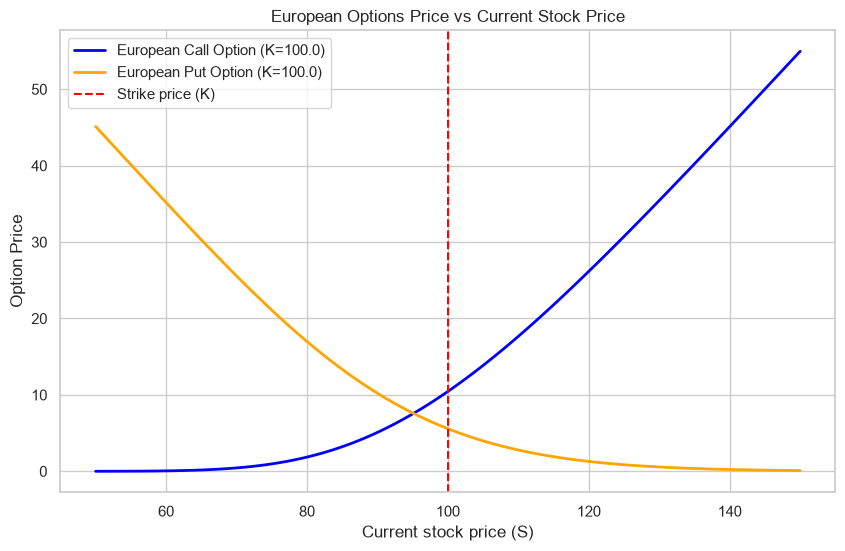
\includegraphics[width=0.8\textwidth]{Figs/bs_graph1.png}
    \caption{Comportamento dos preços das opções europeias de compra e venda
    em função do preço do ativo subjacente.}
    \label{fig:black_scholes_call_put}
    \small Elaborado pelo autor.
\end{figure}
É possível observar a convexidade do preço da opção de compra em relação ao
preço do ativo subjacente. Conforme discutido por Black e Scholes
\cite{blackscholes1973}, a curva que relaciona o valor da opção ao preço
do ativo apresenta curvatura positiva. No modelo de Black--Scholes, essa
propriedade pode ser expressa pela segunda derivada do preço da opção em
relação a $S$,

\begin{equation}
\frac{\partial^2 C}{\partial S^2} = \Gamma > 0.
\end{equation}
No gráfico obtido, esse comportamento pode ser observado pelo aumento
progressivo da inclinação da curva da opção à medida que $S$
aumenta. A relação entre o preço do ativo subjacente $S$ e o preço de exercício $K$
permite classificar a opção quanto ao seu \textit{moneyness}. Para uma opção
de compra (\textit{call}), quando $S<K$, a opção encontra-se
\textit{out of the money} (OTM); quando $S=K$, encontra-se
\textit{at the money} (ATM); e, quando $S>K$, encontra-se
\textit{in the money} (ITM).

Para uma opção de venda (\textit{put}), essa relação ocorre de forma inversa:
quando $S<K$, a opção está ITM; quando $S=K$, está ATM; e, quando $S>K$,
está OTM.

Após a implementação das funções de precificação das opções de compra e
venda, foram implementadas as principais gregas do modelo de
Black--Scholes: Delta, Gamma, Vega, Theta e Rho. Essas medidas representam
as sensibilidades do preço da opção em relação a diferentes parâmetros do
modelo.


Após a implementação das funções de precificação,
foram implementadas as principais Gregas do modelo
de Black--Scholes: Delta, Gamma, Vega, Theta e Rho.

As funções foram desenvolvidas a partir das
expressões analíticas apresentadas na
fundamentação teórica.

Para verificar graficamente o comportamento
dessas sensibilidades em relação ao preço
do ativo subjacente, utilizou-se a mesma
configuração de parâmetros adotada na
análise exploratória anterior, variando-se
$S$ entre 50 e 150.

Os resultados são apresentados na
Figura~\ref{fig:gregas}.

\begin{figure}[H]
    \centering
    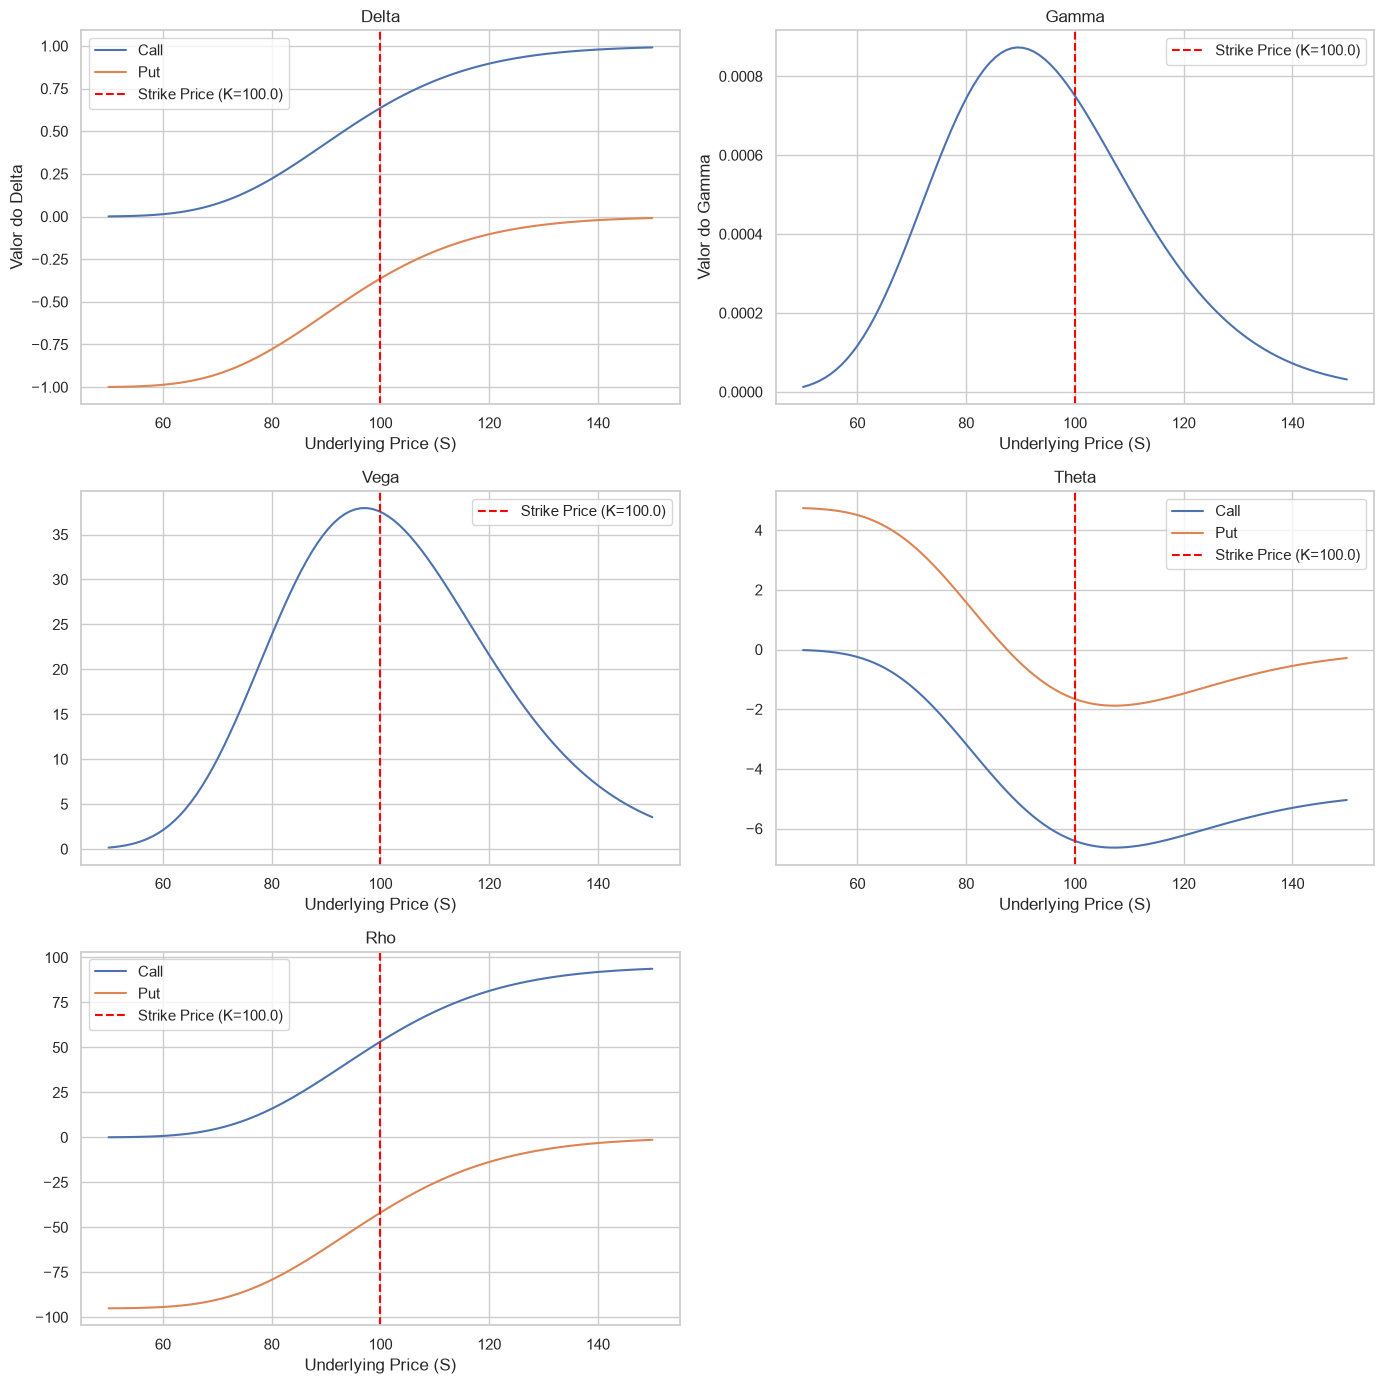
\includegraphics[width=\textwidth]{Figs/gregas.png}
    \caption{Comportamento das gregas em função do preço do ativo subjacente.}
    \label{fig:gregas}
    
    \small Elaborado pelo autor.
\end{figure}
\subsection{Análise Univariada de parâmetros}
Com o objetivo de investigar a capacidade da regressão simbólica de identificar relações matemáticas existentes no modelo de Black--Scholes, foi adotada uma abordagem univariada de cada parâmetro. Essa estratégia consiste em manter um parâmetro da precificação variando e os demais constantes, de modo a isolar cada contribuição para o comportamento do preço da opção. Essa abordagem permite analisar as expressões obtidas pelo PySR em condições controladas, reduzindo a influência simultânea das demais variáveis. Além disso, possibilita comparar as expressões
geradas com as aproximações analíticas apresentadas
na fundamentação teórica, em especial as
expansões de Taylor e de Puiseux. Em todos os casos,
o preço de exercício foi mantido fixo em $K=100$.
Nos experimentos em que $S$ permaneceu constante,
adotou-se $S=100$; nos demais, os parâmetros
fixos foram $r=0{,}05$, $\sigma=0{,}20$ e
$\tau=180/252$, conforme a variável investigada. Nesta etapa, os valores utilizados como referência foram
calculados diretamente pela solução analítica
de Black--Scholes, já implementada e detalhada anteriormente. Para cada experimento, os dados foram organizados
em conjuntos de treinamento e teste, utilizados,
respectivamente, para o ajuste das expressões
simbólicas e para a avaliação de sua capacidade
preditiva. As expressões obtidas foram analisadas
considerando o erro de aproximação, a complexidade
simbólica e a correspondência com as propriedades
matemáticas do modelo de Black--Scholes.

Essa abordagem estabelece uma referência inicial
para a investigação da regressão simbólica,
permitindo distinguir a recuperação de estruturas
matemáticas individuais da aproximação de relações
mais complexas entre múltiplas variáveis.
\subsubsection{Configuração dos Experimentos Univariados}
\subsubsection*{Variação do tempo até o vencimento ($\tau$)}

O primeiro experimento univariado investigou a
dependência do preço de uma opção europeia de compra
em relação ao tempo restante até o vencimento,
$\tau$. Nesse experimento, apenas $\tau$ foi
considerado variável independente, enquanto os
demais parâmetros do modelo de Black--Scholes
permaneceram constantes.

Foram adotados o preço do ativo subjacente
$S=100$, o preço de exercício $K=100$,
a taxa livre de risco $r=0{,}05$ e a
volatilidade $\sigma=0{,}20$.

Para construir o conjunto de dados, foram
considerados 180 valores do tempo restante
até o vencimento, correspondentes aos prazos
de 1 a 180 dias úteis. Esses valores foram
convertidos para anos, utilizando a convenção
de 252 dias úteis, conforme:

\begin{equation}
    \tau_i = \frac{d_i}{252},
    \qquad d_i \in \{1,2,\ldots,180\}.
\end{equation}

Dessa forma, o experimento compreendeu o
intervalo de $\tau \in [1/252,180/252]$.
Para cada valor de $\tau_i$, o preço
teórico da opção foi calculado diretamente
pela formulação analítica de Black--Scholes,
constituindo a variável-alvo do treinamento.

O conjunto resultante foi dividido em
144 observações para treinamento (80\%)
e 36 para teste (20\%). A separação foi
realizada de maneira determinística,
reservando os maiores valores de $\tau$
para treinamento e os menores para teste.

Além dos preços calculados diretamente pela
formulação de Black--Scholes, foram determinados
os coeficientes teóricos da expansão assintótica
em função de $\tau$, considerando a condição \textit{at-the-money} ($S=K$). Para isso, implementou-se uma função em Python
que calcula os coeficientes associados aos
termos $\tau^{1/2}$, $\tau$, $\tau^{3/2}$
e $\tau^2$, conforme a expansão de Puiseux
apresentada na fundamentação teórica. Esses coeficientes foram calculados
independentemente do treinamento do PySR,
sendo utilizados posteriormente como
referência analítica para avaliar a
correspondência entre as expressões obtidas
pela regressão simbólica e a estrutura
assintótica do modelo de Black--Scholes.
A implementação recebe como parâmetros os valores
de $S$, $K$, $r$ e $\sigma$, retornando os
coeficientes associados aos termos
$\tau^{1/2}$, $\tau$, $\tau^{3/2}$ e $\tau^2$,
respectivamente. Resumindamente, em forma de tabela, tem-se:

A Tabela~\ref{tab:parametros_tau} sintetiza os parâmetros
utilizados no primeiro experimento univariado,
destacando a variável investigada e os valores
mantidos constantes.


\begin{table}[htbp]
    \centering
    \caption{Configuração dos parâmetros do experimento univariado com $\tau$.}
    \label{tab:parametros_tau}

    \begin{tabular}{lcc}
        \hline
        \textbf{Parâmetro} &
        \textbf{Condição} &
        \textbf{Valor utilizado} \\
        \hline
        Preço do ativo ($S$) & Constante & $100$ \\
        Preço de exercício ($K$) & Constante & $100$ \\
        Taxa livre de risco ($r$) & Constante & $0{,}05$ \\
        Volatilidade ($\sigma$) & Constante & $0{,}20$ \\
        Tempo até o vencimento ($\tau$) &
        Variável & $[1/252,\;180/252]$ ano \\
        \hline
        Total de observações & --- & $180$ \\
        Treinamento & 144 observações &
        $\tau \in [37/252,\;180/252]$ \\
        Teste & 36 observações &
        $\tau \in [1/252,\;36/252]$ \\
        \hline
    \end{tabular}

    \vspace{0.2cm}
    {\footnotesize Fonte: Elaboração própria.\par}
\end{table}


A precisão das expressões identificadas pelo PySR
foi avaliada por meio do erro absoluto médio
(MAE), do erro quadrático médio (MSE) e da raiz
do erro quadrático médio (RMSE).

Essas métricas foram calculadas sobre os conjuntos
de teste, considerando como referência os preços
obtidos pela formulação analítica de Black--Scholes. Além da avaliação preditiva, foram consideradas
a complexidade simbólica das expressões e sua
correspondência com as propriedades matemáticas
do modelo de referência, incluindo os coeficientes
das expansões de Taylor e de Puiseux.

\subsubsection*{Variação da taxa de juros ($r$)}
O segundo experimento univariado investigou a dependência
do preço de uma opção europeia de compra em relação à taxa
livre de risco, $r$. Nesse experimento, apenas a taxa de
juros foi considerada variável independente, enquanto
os demais parâmetros do modelo de Black--Scholes
permaneceram constantes. Foram adotados o preço do ativo subjacente $S=100$,
o preço de exercício $K=100$, a volatilidade
$\sigma=0{,}20$ e o tempo restante até o vencimento
$\tau=180/252$ ano. Para a construção do conjunto de dados, foram
considerados 91 valores da taxa livre de risco,
distribuídos uniformemente no intervalo de
$0{,}01$ a $0{,}10$, com incrementos de $0{,}001$.
Assim, os valores da variável independente
foram definidos por:

\begin{equation}
r_i = 0{,}01 + 0{,}001i,
\qquad i \in \{0,1,\ldots,90\}.
\end{equation}

Essa separação determinística permitiu avaliar
a capacidade de extrapolação das expressões
simbólicas para taxas superiores às utilizadas
durante o treinamento.

Além da avaliação dos preços calculados pelo
PySR, foram determinados os coeficientes
teóricos da expansão de Taylor de segunda
ordem da função de Black--Scholes em relação
à taxa livre de risco, considerando como
ponto de expansão $r_0=0$.

A aproximação analítica foi expressa por:

\begin{equation}
C_{BS}(r) =
a_0 + a_1r + a_2r^2 + \mathcal{O}(r^3),
\end{equation}

em que $a_0$ corresponde ao preço teórico
da opção em $r=0$, $a_1$ representa a
primeira derivada do preço em relação à
taxa livre de risco, associada à sensibilidade
Rho, e $a_2$ corresponde à metade da
segunda derivada em relação a $r$. Ressalta-se que os preços utilizados no treinamento
foram obtidos pela formulação analítica exata
de Black--Scholes, enquanto a expansão de Taylor
foi empregada exclusivamente na comparação
das propriedades matemáticas das expressões
identificadas. A tabela ~\ref{tab:parametros_r} abaixo mostra um resumo dos parâmetros.


\begin{table}[htbp]
    \centering
    \caption{Configuração do experimento univariado
    com a taxa livre de risco ($r$).}
    \label{tab:parametros_r}

    \begin{tabular}{lcc}
        \hline
        \textbf{Parâmetro} &
        \textbf{Condição} &
        \textbf{Valor utilizado} \\
        \hline
        Preço do ativo ($S$) & Constante & $100$ \\
        Preço de exercício ($K$) & Constante & $100$ \\
        Volatilidade ($\sigma$) & Constante & $0{,}20$ \\
        Tempo até o vencimento ($\tau$) &
        Constante & $180/252$ ano \\
        Taxa livre de risco ($r$) &
        Variável & $[0{,}01;\,0{,}10]$ \\
        Incremento de $r$ & --- & $0{,}001$ \\
        \hline
        Total de observações & --- & $91$ \\
        Treinamento & 71 observações &
        $r \in [0{,}01;\,0{,}08]$ \\
        Teste & 20 observações &
        $r \in [0{,}081;\,0{,}10]$ \\
        \hline
    \end{tabular}

    \vspace{0.2cm}
    {\footnotesize Fonte: Elaboração própria.\par}
\end{table}

\subsubsection*{Variação da volatilidade ($\sigma$)}
O terceiro experimento univariado teve como objetivo
investigar a capacidade da regressão simbólica de
aproximar a relação entre a volatilidade e o preço
de uma opção europeia de compra, mantendo constantes
os demais parâmetros do modelo de Black--Scholes. Foram adotados $S=K=100$, taxa livre de risco
$r=0{,}05$ e tempo restante até o vencimento
$\tau=180/252$ ano. Para a construção do conjunto de dados, foram
considerados 31 valores de volatilidade,
igualmente espaçados entre $0{,}10$ e $0{,}40$,
com incrementos de $0{,}01$. Para cada valor
de $\sigma$, o preço teórico da opção foi
calculado diretamente pela formulação analítica
de Black--Scholes, constituindo a variável-alvo
do experimento.

O conjunto de dados foi ordenado de maneira
crescente em relação à volatilidade e dividido
em 24 observações para treinamento e 7 para
teste. O treinamento compreendeu valores de
$\sigma$ entre $0{,}10$ e $0{,}33$, enquanto
o conjunto de teste contemplou valores entre
$0{,}34$ e $0{,}40$. Essa divisão determinística
permitiu avaliar a capacidade de extrapolação
das expressões identificadas pelo PySR para
volatilidades superiores às observadas durante
o treinamento. Além da avaliação da precisão dos preços
estimados, foram determinados os coeficientes
teóricos da expansão de Taylor de segunda
ordem da função de Black--Scholes em relação
à volatilidade, considerando como ponto de
expansão $\sigma_0=0{,}20$.

A aproximação analítica foi expressa por:

\begin{equation}
\begin{aligned}
C_{BS}(\sigma) \approx {}&
a_0+a_1(\sigma-\sigma_0)\\
&+a_2(\sigma-\sigma_0)^2,
\end{aligned}
\end{equation}

em que $a_0$ corresponde ao preço da opção
no ponto de expansão, $a_1$ representa
a primeira derivada em relação à volatilidade
(Vega) e $a_2$ corresponde à metade da
segunda derivada em relação à volatilidade
(Vomma).
Para os parâmetros fixados, os coeficientes
teóricos calculados foram:

\begin{equation}
\begin{aligned}
C_{BS}(\sigma) \approx {}&
8{,}518175855\\
&+32{,}273470128(\sigma-0{,}20)\\
&+3{,}025637825(\sigma-0{,}20)^2.
\end{aligned}
\end{equation}

Esses coeficientes foram obtidos
independentemente do treinamento do PySR,
por meio de uma função implementada em Python.
A expansão foi utilizada como referência
para investigar se as expressões simbólicas
identificadas reproduzem o comportamento
local da função de precificação, incluindo
sua sensibilidade e curvatura em relação
à volatilidade. A Tabela~\ref{tab:parametros_sigma} apresenta um resumo
dos parâmetros utilizados no experimento em que
a volatilidade ($\sigma$) é variável.


\begin{table}[htbp]
    \centering
    \caption{Configuração dos parâmetros do experimento univariado com $\sigma$.}
    \label{tab:parametros_sigma}

    \begin{tabular}{lcc}
        \hline
        \textbf{Parâmetro} &
        \textbf{Condição} &
        \textbf{Valor utilizado} \\
        \hline
        Preço do ativo ($S$) & Constante & $100$ \\
        Preço de exercício ($K$) & Constante & $100$ \\
        Taxa livre de risco ($r$) & Constante & $0{,}05$ \\
        Tempo até o vencimento ($\tau$) &
        Constante & $180/252$ ano \\
        Volatilidade ($\sigma$) &
        Variável & $[0{,}10;\,0{,}40]$ \\
        Incremento de $\sigma$ & --- & $0{,}01$ \\
        \hline
        Total de observações & --- & $31$ \\
        Treinamento & 24 observações &
        $\sigma \in [0{,}10;\,0{,}33]$ \\
        Teste & 7 observações &
        $\sigma \in [0{,}34;\,0{,}40]$ \\
        \hline
    \end{tabular}

    \vspace{0.2cm}
    {\footnotesize Fonte: Elaboração própria.\par}
\end{table}


% Impede que as tabelas dos experimentos ultrapassem esta subseção.
\FloatBarrier
\subsubsection*{Variação do preço do ativo ($S$)}
O experimento univariado com o preço do ativo subjacente  
teve como objetivo investigar a capacidade da regressão simbólzica de aproximar a função de precificação de Black--Scholes quando apenas a variável $S$ é modificada. Para isso, foram mantidos constantes o preço de exercício $K=100$, a taxa livre de risco $r=0{,}05$, a volatilidade $\sigma=0{,}20$ e o tempo restante até o vencimento $\tau=180/252$ ano.

O \textit{dataset} foi construído a partir de 91 valores igualmente espaçados de ($S$), compreendidos entre 70 e 130. Para cada observação, o preço teórico da opção europeia de compra foi calculado diretamente pela formulação analítica de Black-Scholes, constituindo a variável-alvo do treinamento. Os dados foram ordenados de maneira crescente e particionados deterministicamente em 71 observações de treinamento e 20 de teste, correspondentes, respectivamente, aos intervalos de aproximadamente 70 a 116,67 e de 117,33 a 130. Essa divisão foi adotada para avaliar a capacidade de extrapolação das expressões simbólicas para preços do ativo superiores aos utilizados durante o ajuste.
Como uma primeira rodade de testes, realizou-se o treinamento utilizando a configuração padrão estabelecida para os experimentos univariados, com 500 iterações, operadores binários de adição, subtração, multiplicação e divisão, e operadores unários exponencial, logaritmo, raiz quadrada e função erro (\textit{erf}). O tamanho máximo das expressões foi limitado a 35, utilizando-se o critério \texttt{model\_selection=best} para a seleção automática de uma expressão pelo PySR.

A investigação foi organizada em duas rodadas independentes de treinamento do PySR, diferenciadas pela configuração dos hiperparâmetros responsáveis pela exploração do espaço de busca simbólica. Em ambas, foram utilizados os mesmos conjuntos de treinamento e teste, mantendo-se ($S$) como a única variável independente.

Na primeira rodada de treinamento, adotou-se a configuração inicial estabelecida para os experimentos univariados, com 500 iterações, operadores binários de adição, subtração, multiplicação e divisão, além dos operadores unários exponencial, logaritmo, raiz quadrada e função erro (erf). O tamanho máximo das expressões foi limitado a 35, utilizando-se o critério \texttt{model\_selection="best"} para a seleção automática de uma expressão pelo PySR. Após o treinamento, as expressões preservadas pelo algoritmo foram avaliadas quanto à precisão preditiva nos conjuntos de treinamento e teste, considerando também sua complexidade simbólica.

Na segunda rodada, realizou-se um novo treinamento independente, com uma configuração ampliada de hiperparâmetros, visando investigar a influência de uma busca evolutiva mais extensa sobre as expressões identificadas. Nessa execução, o número de iterações foi aumentado para 1.200, com 24 populações e 40 indivíduos por população. Também foram definidos 500 ciclos evolutivos por iteração, tamanho máximo de expressão igual a 40 e profundidade máxima igual a 12. Os operadores matemáticos e o critério de seleção foram mantidos em relação à primeira rodada, sendo utilizada a semente aleatória \texttt{random\_state=42}. Adicionalmente, foi realizada uma análise da correspondência entre as expressões simbólicas e as propriedades analíticas do modelo de Black-Scholes. Para isso, considerou-se a expansão teórica de Taylor de segunda ordem em relação a $S$, em torno do ponto ($S_0=100$). Para cada expressão selecionada para análise, foram calculados seu valor, sua primeira derivada e a segunda derivada no ponto de expansão, permitindo a comparação com o preço teórico da opção, Delta e metade de Gamma.

De maneira complementar, as derivadas das expressões foram avaliadas em uma malha de 301 pontos no intervalo de ($S=70$) a ($S=130$). Esse procedimento permitiu investigar a correspondência com as sensibilidades analíticas de Black-Scholes e verificar a preservação de propriedades matemáticas, como monotonicidade, limites de Delta e convexidade.

Para a avaliação das expressões, foram considerados o erro absoluto médio (MAE), o erro quadrático médio (MSE), a raiz do erro quadrático médio (RMSE) e a complexidade simbólica ,ou seja seu sentido matemático e financeiro , esta análise de desempenho considerou tanto a interpretabilidade no domínio do problema, atestada pelo comportamento das Gregas, quanto a eficiência matemática. Além da expressão selecionada automaticamente pelo algoritmo, foram examinadas outras expressões preservadas pelo PySR, permitindo investigar diferentes compromissos entre precisão numérica e sentido financeiro e matemático. Abaixo uma tabela resumindo quais fora os hiper parâmetros usados nos experimentos.


\begin{table}[htbp]
    \centering
    \caption{Configurações dos hiperparâmetros duas execuções do PySR
    para a variação do preço do ativo subjacente.}
    \label{tab:configuracoes_pysr_S}

    \begin{tabular}{lcc}
        \hline
        \textbf{Hiperparâmetro} &
        \textbf{Inicial} &
        \textbf{Ampliada} \\
        \hline
        \texttt{niterations} & 500 & 1200 \\
        \texttt{populations} & 31 & 24 \\
        \texttt{population\_size} & 27 & 40 \\
        \texttt{ncycles\_per\_iteration} & 380 & 500 \\
        \texttt{maxsize} & 35 & 40 \\
        \texttt{maxdepth} & \texttt{None} & 12 \\
        \texttt{model\_selection} & best & best \\
        \texttt{random\_state} & \texttt{None} & 42 \\
        \hline
    \end{tabular}

    \vspace{0.2cm}
    {\footnotesize Fonte: Elaboração própria.\par}
\end{table}
A seguir, a Tabela~\ref{tab:parametros_S} resume a dinâmica desta rodada de testes em relação ao preço do ativo $S$.
\begin{table}[H]
    \centering
    \caption{Configuração dos parâmetros do experimento univariado com $S$.}
    \label{tab:parametros_S}
    
    \begin{tabular}{lcc}
        \hline
        \textbf{Parâmetro} & \textbf{Condição} & \textbf{Valor utilizado} \\
        \hline
        Preço do ativo ($S$) & Variável & $[70;130]$ \\
        Preço de exercício ($K$) & Constante & 100 \\
        Taxa livre de risco ($r$) & Constante & 0,05 \\
        Tempo até o vencimento ($\tau$) & Constante & $180/252$ ano \\
        Volatilidade ($\sigma$) & Constante & 0,20 \\
        Incremento de $S$ & --- & $2/3 \approx 0,6667$ \\
        \hline
        \textbf{Total de observações} & --- & \textbf{91} \\
        \hline
        Treinamento & 71 observações & $S \in [70;116,67]$ \\
        Teste & 20 observações & $S \in [117,33;130]$ \\
        \hline
    \end{tabular}

    \vspace{0.2cm}
    {\footnotesize Fonte: Elaboração própria.\par}
\end{table}

\subsection{Configuração da Regressão Simbólica}

\subsection{Procedimento Experimental}

\subsection{Métricas de Avaliação}
   % Metodologia

\section{Resultados e Discussão}


Este capítulo apresenta e discute os resultados obtidos
nos experimentos de regressão simbólica realizados com
o PySR, utilizando como referência os preços calculados
pela formulação analítica de Black--Scholes.

A análise considera a precisão preditiva, a complexidade
das expressões identificadas e sua correspondência com
as propriedades matemáticas do modelo original.


\subsection{Resultados dos Experimentos Univariados}
\label{sec:resultados_univariados}

Nesta etapa, são analisados os resultados obtidos pela
variação individual dos parâmetros de Black--Scholes,
mantendo-se os demais constantes.

As expressões identificadas pelo PySR são comparadas
com as expansões analíticas apresentadas na fundamentação
teórica, buscando investigar a recuperação de estruturas
matemáticas e a precisão das aproximações.


\subsection{Tempo Restante até o Vencimento ($\tau$)}
\label{subsec:resultados_tau}

% 1. Apresentação da expressão selecionada pelo PySR
% 2. Equações 6, 14 e 16
% 3. Comparação com a expansão de Puiseux
% 4. Tabela dos coeficientes teóricos e encontrados
% 5. Comparação dos erros e complexidades
% 6. Discussão dos resultados


\subsection{Taxa Livre de Risco ($r$)}
\label{subsec:resultados_r}

% 1. Expressão selecionada pelo PySR
% 2. Equações 8, 10, 14 e demais relevantes
% 3. Comparação com a expansão de Taylor
% 4. Tabela dos coeficientes
% 5. MAE, MSE, RMSE e complexidade
% 6. Discussão da recuperação estrutural


\subsection{Volatilidade ($\sigma$)}
\label{subsec:resultados_sigma}

% 1. Expressão selecionada pelo PySR
% 2. Equações 5, 14 e 15
% 3. Comparação com a expansão de Taylor
% 4. Análise dos coeficientes teóricos
% 5. Comparação preditiva
% 6. Análise das sensibilidades Vega e Vomma


\subsection{Preço do Ativo Subjacente ($S$)}
\label{subsec:resultados_S}

% 1. Expressão selecionada pelo PySR
% 2. Equações relevantes
% 3. Comparação com a expansão de Taylor
% 4. Análise dos coeficientes teóricos
% 5. Avaliação preditiva
% 6. Análise das sensibilidades Delta e Gamma


\section{Discussão Comparativa dos Experimentos Univariados}
\label{sec:discussao_univariados}

% Comparação da recuperação estrutural
% Relação entre complexidade simbólica e erro
% Diferenças entre ajuste local e extrapolação
% Limitações das expressões encontradas


\section{Experimentos Multivariados}
\label{sec:resultados_multivariados}

% Inserir os resultados dos experimentos
% com mais de uma variável independente.
% Preservar aqui as análises com trajetórias
% de Monte Carlo, quando forem discutidas.


\section{Síntese dos Resultados e Limitações}
\label{sec:sintese_resultados}

% Principais resultados
% Limitações metodológicas
% Alcance das conclusões


\include{resultados}    % Experimentos e Resultados

\section{ Conclusões}
\label{chapter:conclusions}    % Conclusão


{
\thispagestyle{empty}
\renewcommand{\refname}{REFERÊNCIAS}
\bibliography{bibliografia}
}

\newpage

\end{document}